\documentclass[11pt, a4paper, openany]{book}

\usepackage[bottom=0.9in,top=0.9in, left=0.9in, right=0.9in]{geometry}

\usepackage{graphicx}
\usepackage{xcolor}
\usepackage{amsmath}
\usepackage{titlesec}
\usepackage{hyperref}
\newenvironment{abstract}{}{}
\usepackage{abstract}
\usepackage{listings}
\usepackage{newlfont}
\usepackage{color}


\usepackage{afterpage}

\newcommand\blankpage{%
	\null
	\thispagestyle{empty}%
	\addtocounter{page}{-1}%
	\newpage}
\renewcommand\bibname{Bibliografia e Immagini}

\newcommand{\toask}[1]{\color{red}#1}



\titlespacing*{\section}
{0pt}{12ex plus 1ex minus .7ex}{4.3ex plus .2ex}

\begin{document}
		
	\begin{titlepage}
		\begin{center}
			{{\Large{\textsc{Alma Mater Studiorum $\cdot$ Universit\`a di Bologna}}} \\ \large Campus di Cesena} 
			\rule[0.1cm]{15.8cm}{0.1mm}
			\rule[0.5cm]{15.8cm}{0.6mm}
			\\\vspace{3mm}
			
			{\small{ DIPARTIMENTO DI INFORMATICA – SCIENZA E INGEGNERIA \\ 
					Corso di Laurea in Ingegneria e Scienze Informatiche}}
			
		\end{center}
		
		\vspace{23mm}
		
		\begin{center}\textcolor{black}{
				{\LARGE{\bf WebRTC: studio della tecnologia e casi d'uso}}\\
		}\end{center}
		
		\vspace{25mm}
		
		\begin{center}
			{\Large Elaborato in:\\
			Programmazioni di reti}
		\end{center}
		
		\vspace{25mm} \par \noindent
		
		\begin{minipage}[t]{0.47\textwidth}
			{\large{\bf Relatore: \vspace{2mm}\\\textcolor{black}{
						Prof. Andrea Piroddi}}}
		\end{minipage}
		\hfill
		\begin{minipage}[t]{0.47\textwidth}\raggedleft \textcolor{black}{
				{\large{\bf Presentata da:\vspace{2mm}\\Giovanni Maffi}}}
		\end{minipage}
		
		\vspace{40mm}
		
		\begin{center}
			Anno Accademico \textcolor{black}{2022/2023}
		\end{center}
		
	\end{titlepage}
	
	\afterpage{\blankpage}
	
	\begin{flushright}
		\thispagestyle{empty} 
		\vspace*{100mm}
		\Large \emph{"Sic Mundus Creatus Est"}
	\end{flushright}
	
	\afterpage{\blankpage}
	
	\tableofcontents 

	\afterpage{\blankpage}
	
%	\begin{abstract}
%		In questo documento viene analizzato WebRTC, una nuova tecnologia che rinnova le comunicazioni real-time tra più utenti tramite il solo utilizzo di un browser, permettendo di effettuare videochiamate. Il suo utilizzo si espande anche in altri ambienti, come quello del controllo remoto di dispositivi, utile per esempio per monitorare il funzionamento di macchinari. Verrà analizzato anche un progetto che permette di effettuare una chiamata tra un dottore e un paziente.
%	\end{abstract}

	\afterpage{\blankpage}
	\chapter{Introduzione}
	
	Negli ultimi 150 anni l'uomo ha fatto passi da gigante nel settore tecnologico/informatico con alcune invenzioni così importanti da cambiare il suo modo di vivere: basti pensare alla televisione presente in ogni casa, all'evoluzione dei computer e degli smartphone e, soprattutto, ad Internet che ha permesso all'uomo di informarsi su un qualsiasi argomento e di interagire con tutti in tempo reale. A tal proposito, la possibilità di comunicare in tempo reale con altri utenti è possibile grazie all'utilizzo di vari protocolli che, però, richiedono sempre l'utilizzo di plugin o software esterni. Nonostante ciò, negli ultimi anni è stata creata e sviluppata una nuova tecnologia che permette una comunicazione in tempo reale senza l'utilizzo di elementi terzi ed è sempre più discussa ed utilizzata: si tratta di WebRTC (Web Real-Time Communication).

 	\afterpage{\blankpage}
 	\chapter{Storia}
 	\section{La nascita della comunicazione in tempo reale}
 	Nonostante WebRTC esista da poco più di 10 anni, la comunicazione a distanza nasce più di un secolo fa, con l'invenzione della telefonia. La nascita del telefono risale alla seconda metà del XIX secolo, anche se la paternità di tale invenzione è ancora oggi contestata (tra i tanti possibili inventori, i più accreditati sono Antonio Meucci, Innocenzo Manzetti, Johann Philipp Reis, Alexander Graham Bell e Charles Bourseul) \cite{1}. il suo utilizzo, però, si diffuse più tardi, intorno agli anni '20, ed è proprio in questi anni che nascono i primi servizi di telecomunicazione. Col passare degli anni, i telefoni sono diventati sempre più sofisticati e diversificati. Verso la fine degli anni ‘80 si assiste ad una progressiva comparsa dei telefoni portatili, che porteranno sempre di più al disuso dei telefoni fissi \cite{2}.
 	\begin{figure}[h!]
 		\centering
 		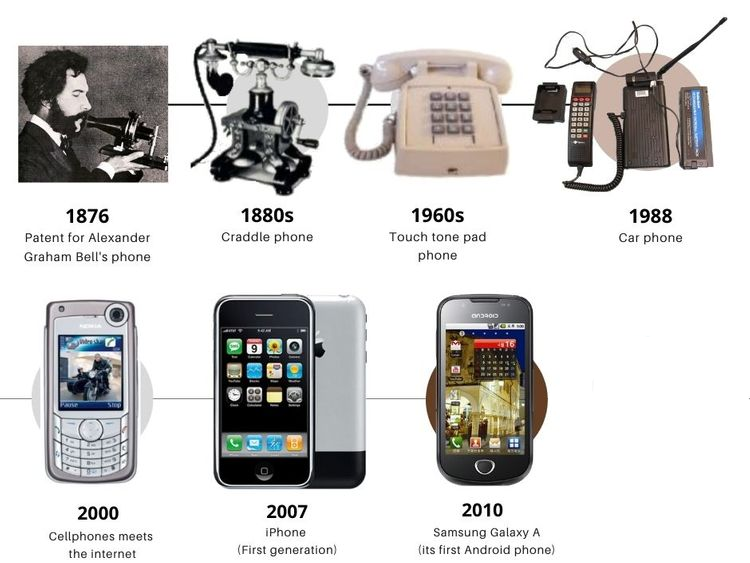
\includegraphics[width=0.7\textwidth]{img/TelEvo.png}
 		\caption{Evoluzione della telefonia \cite{55}.}
 	\end{figure}
 	\newpage

 	\section{VoIP}
 	La nascita di Internet ha cambiato notevolmente la comunicazione in tempo reale, permettendo lo streaming non solo di audio, ma anche di contenuto multimediale. La tecnologia più importante tra tutte è sicuramente VoIP. $\\$
 	VoIP (Voice over Internet Protocol) è un insieme di tecnologie che permette la comunicazione tra due o più utenti, sfruttando il protocollo IP per il trasporto dati.  $\\$
 	Una tecnologia VoIP opera trasferendo segnali vocali tra indirizzi IP, il che significa che questi segnali devono essere codificati in pezzi di dati abbastanza piccoli da poter essere trasmessi. I campioni vocali del mittente vengono suddivisi in "pacchetti" vocali a cui sono fornite informazioni di instradamento e inviati al destinatario. I pacchetti vengono trasmessi uno ad uno, quindi si riformano il più vicino possibile allo stato originale, creando un'unica voce. Questo processo comprime il segnale vocale e quindi decomprime il segnale per il ricevitore \cite{3}. $\\$
 	Il primo utilizzo di VoIP risale al 1995 quando VocalTec Communication, un’azienda israeliana, brevetta il primo trasmettitore Voice over IP. Le basse velocità di connessione, però, significavano scarsa qualità audio, chiamate frequentemente interrotte e grave latenza e perdita di pacchetti. Questi problemi hanno impedito a VoIP di diffondersi in quegli anni; infatti la sua notorietà è avvenuta negli ultimi 20 anni, grazie alla creazione di tante applicazioni che utilizzano queste tecnologie per la comunicazione in tempo reale. Prima fra tutte è Skype: nato nel 2003 e pensato inizialmente come software per effettuare semplici chiamate, è stata la prima applicazione che, tramite l'utilizzo di voip, ha permesso la possibilità di attuare delle videochiamate; successivamente sono nate molte altre applicazioni simili e molte di queste hanno guadagnato una grande fama durante gli anni della pandemia di Covid \cite{4}. $\\$
	\begin{figure}[h!]
		\centering
		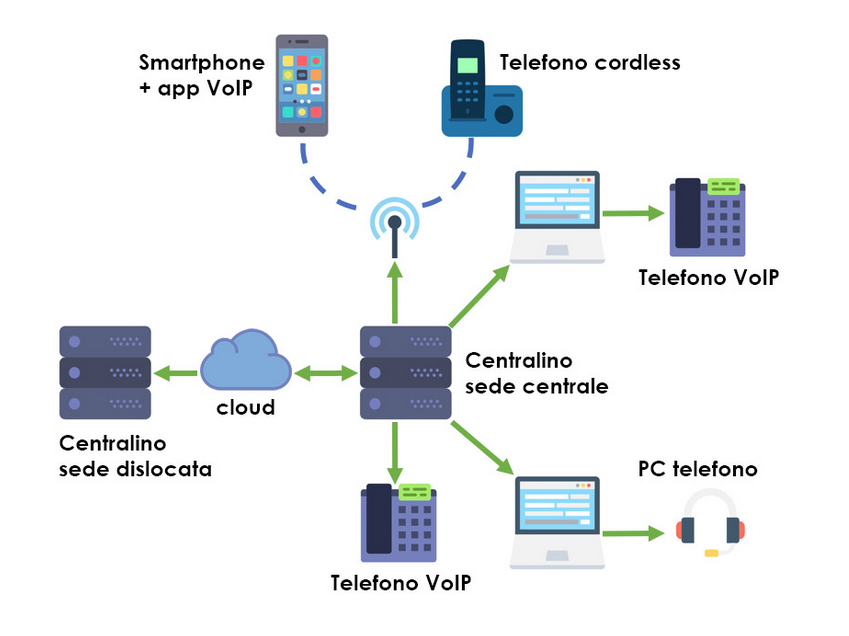
\includegraphics[width=0.7\textwidth]{img/VoIP.png}
		\caption{VoIP \cite{56}.}
	\end{figure}
	

 	\newpage
 	\section{RTMP}
 	Real-Time Messaging Protocol (RTMP) è un protocollo di comunicazione creato da Adobe per lo streaming di audio, video e dati su Internet. Creato da Macromedia (acquistato da Adobe), Il suo compito iniziale era quella di trasmettere i dati tra un server e Flash Player (un software per la visualizzazione di contenuti multimediali e l'esecuzione di applicazioni Internet avanzate, utilizzato per creare giochi o interi siti web). Nel corso degli anni, quest'ultimo è diventato sempre più conosciuto ed utilizzato, quindi anche RTMP aveva trovato largo impiego. Nonostante nel dicembre 2020 Adobe Flash Player sia stato dismesso, RTMP viene utilizzato ancora oggi come protocollo per lo streming \cite{5}.  $\\$
 	La versione standard di RTMP prevede l’uso di TCP come protocollo di trasporto. Per prima cosa, client e server effettuano un handshake, scambiandosi tutte le informazioni riferenti alle regole della connessione (sistemi di criptazione, velocità, controllo errori ed altro). Una volta che il server conferma di aver ricevuto i blocchi di dati, può essere stabilita la connessione. A tale scopo, il client invia al server una richiesta di connessione sotto forma di action message (formato utilizzato per serializzare oggetti grafici come xml), dopodiché attende una conferma da parte del server. Quando l’ha ricevuta, il client può avviare lo streaming in tempo reale. Si stabilisce così una connessione stabile grazie alla quale i dati possono essere trasmessi in tempo reale. Per trasmetterli senza intoppi, RTMP suddivide lo stream in frammenti di dimensioni diverse. Queste possono essere "negoziate" tra client e server, altrimenti le dimensioni predefinite dei frammenti sono 64 byte per i dati audio e 128 byte per i dati video e la maggior parte degli altri tipi di dati \cite{5}.$\\$
 	Un programma che supporta questo protocollo è OBS, un software open source utilizzato per la registrazione di video, ma anche per lo streaming tramite RTMP \cite{6}.
 	
 	 	
 	\section{Il problema}
 	Come già detto, nel corso degli anni 2000 queste tecnologie (in particolare quelle VoIP) diventavano sempre più note ed utilizzate, ma il loro impiego non era possibile tramite web, quindi era necessario l'installazione di plugin (per esempio le prime versioni di Google Hangouts) o software (Skype). Tutto ciò fù risolto nel 2011, con la creazione di WebRTC.
 	
 	\newpage
 	
 	\section{WebRTC}
 	Nel maggio 2010, Google acquistò GIPS (Global IP Solutions), una società di software VoIP e videoconferenza che aveva sviluppato molti componenti necessari per RTC, come vari codec (un software o un dispositivo che si occupa della codifica e/o decodifica digitale) e tecniche di cancellazione dell'eco. Successivamente, Google rese open source le tecnologie sviluppate da GIPS e si impegnò con gli organismi di standardizzazione pertinenti dell'IETF e del W3C per garantire il consenso del settore. Nel maggio 2011, Google rilasciò un progetto open source per la comunicazione in tempo reale basata su browser noto come WebRTC. Questo fu seguito da un lavoro per standardizzare i protocolli pertinenti nell'IETF e le API del browser nel W3C \cite{7}. $\\$
 	La prima implementazione avvenne sempre nel maggio del 2011, quando Ericsson Labs (multinazionale svedese operante nella fornitura di tecnologie e servizi di comunicazione, software e infrastrutture) ha creato la prima implementazione di WebRTC utilizzando una libreria WebKit modificata.  $\\$
 	Nel corso degli anni i vari browser hanno iniziato a supportare l'utilizzo di WebRTC, ma l'impiego di questa tecnologia tra browser diversi è stato un problema difficile da risolvere, in particolare con tutti i browser compatibili con iOS, infatti il primo a supportare WebRTC è stato Safari nel 2017 \cite{8}. $\\$
 	Nell'ottobre 2011, il W3C ha pubblicato la sua prima bozza per la specifica. Le pietre miliari di WebRTC includono la prima videochiamata cross-browser (febbraio 2013), i primi trasferimenti di dati cross-browser (febbraio 2014) e, a partire da luglio 2014, Google Hangouts inizia ad utilizzare WebRTC \cite{7}.$\\$
 	\begin{figure}[h!]
 		\centering
 		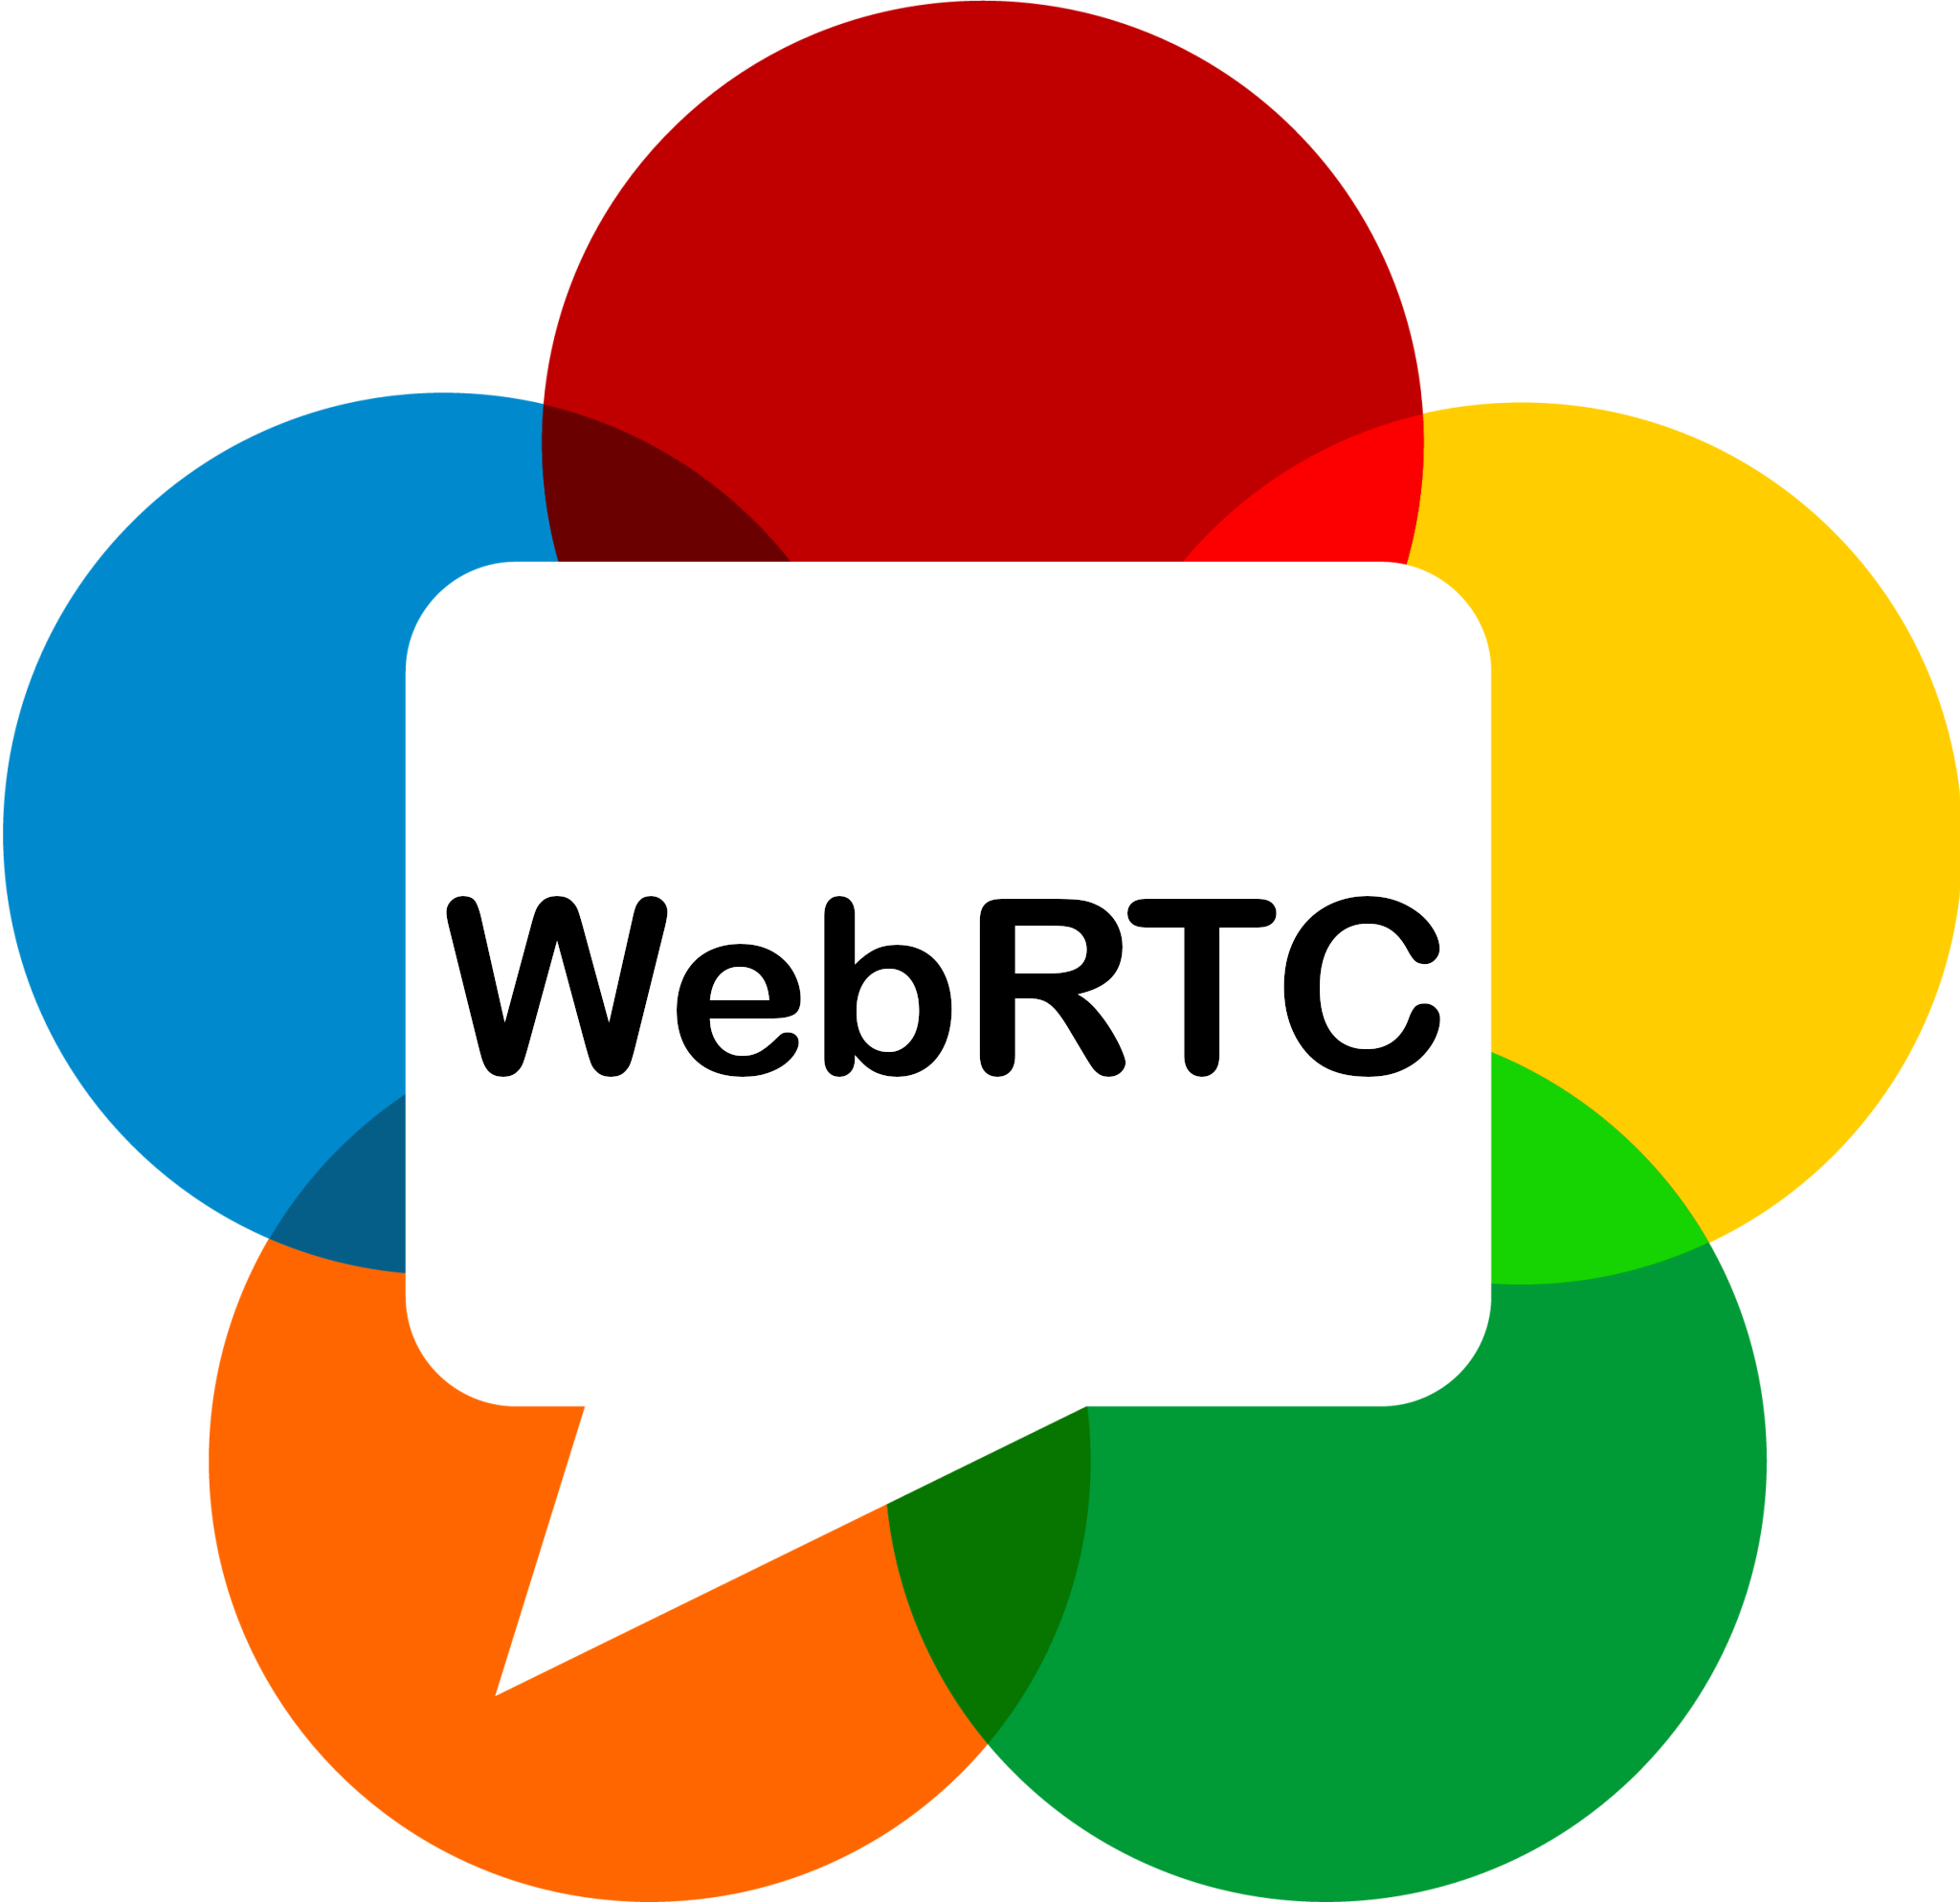
\includegraphics[width=0.5\textwidth]{img/logoWebRTC.png}
 		\caption{Logo di WebRTC \cite{57}.}
 	\end{figure}
 	
 	\newpage
 	
 	\section{WebSocket}
 	WebSocket è una tecnologia web nata nel 2008 che fornisce canali di comunicazione full-duplex attraverso una singola connessione TCP. $\\$
 	Il protocollo WebSocket consente l'interazione tra un browser Web (o un'altra applicazione client) e un server Web con un sovraccarico inferiore rispetto alle alternative half-duplex, facilitando il trasferimento dei dati in tempo reale da e verso il server. WebSocket, inoltre, permette un'interazione maggiore tra browser e server rispetto ad altri protocolli, facilitando la realizzazione di applicazione che forniscono contenuti in tempo reale. Tutto questo è possibile perché il server può spedire informazioni al browser senza aver ricevuto prima una richiesta dal client e consentendo il passaggio dei messaggi avanti e indietro mantenendo la connessione aperta \cite{9}. 
 	
 	\subsection{WebRTC e WebSocket}
	Solitamente si può fare confusione tra queste due tecnologie. Entrambe possono essere utilizzate per lo stesso scopo, ma tra di loro ci sono varie differenze, tra le quali le principali sono \cite{10}:
	\begin{itemize}
		\item WebSocket fornisce un protocollo di comunicazione computer client-server, mentre WebRTC offre un protocollo peer-to-peer e funzionalità di comunicazione per browser e app mobili.
		\item WebSocket è una scelta migliore quando l'integrità dei dati è fondamentale, in quanto si beneficia dell'affidabilità sottostante del TCP. D'altra parte, se la velocità è più importante e la perdita di alcuni pacchetti è accettabile, WebRTC su UDP è una scelta migliore.
	\end{itemize}
 	Nonostante ciò, vedremo come WebSocket venga utilizzato per il funzionamento di WebRTC nella fase di signaling. 
	
	\afterpage{\blankpage}
	
	\chapter{Struttura e Funzionamento di WebRTC}
 	\section{Architettura}
 	 Come già detto, WebRTC offre agli sviluppatori di applicazioni Web la possibilità di scrivere app multimediali e in tempo reale sul Web, senza richiedere plug-in, download o installazioni. L'architettura complessiva la seguente \cite{11}:
 	\begin{figure}[h!]
 		\centering
 		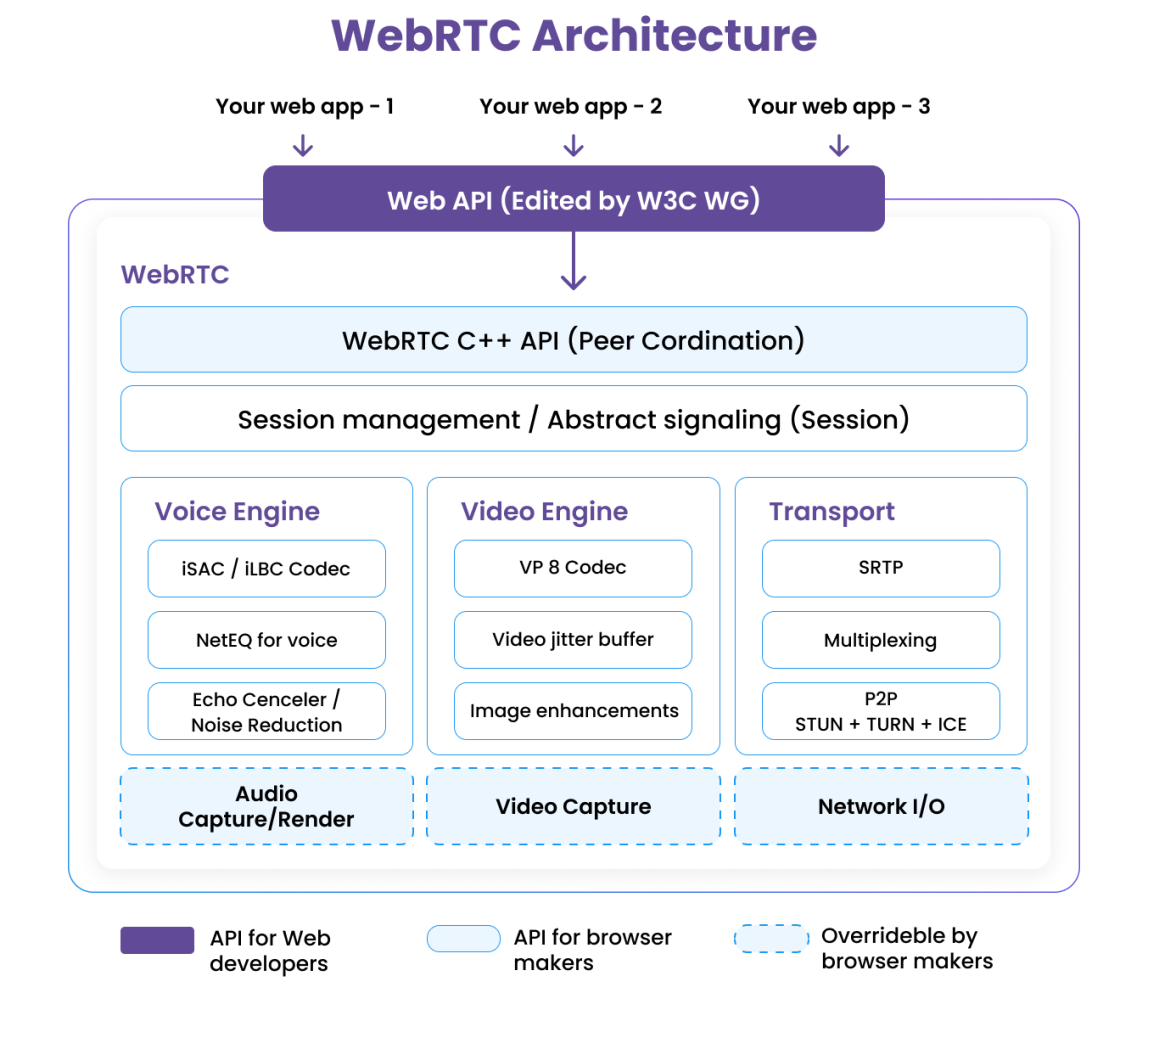
\includegraphics[width=0.7\textwidth]{img/architecture.PNG}
 		\caption{Architettura di WebRTC \cite{58}.}
 	\end{figure}
 	\newpage
 	Come si nota dalla figura 3.1, l'architettura si può dividere in due livelli:
 	\begin{itemize}
 		\item il livello per gli sviluppatori di applicazioni Web, il Web API, l'insieme delle API che viene utilizzato da sviluppatori per la creazione di applicazioni simili a videochat basate sul Web. Alcuni esempi di API sono RTCPeerConnection, RTCDataChannel, e MediaStream.
 		\item Il livello API per gli sviluppatori di browser, in cui è presente l'API WebRTC C++, consente ai produttori di browser di implementare facilmente la proposta di Web API. Qui sono presenti anche delle API sovrascrivibili. 
 	\end{itemize}
 	Il livello transport gestisce l'ordine e la perdita dei pacchetti e si occupa di stabilire e mantenere connessioni tra reti di diverso tipo; per farlo, vengono impiegate le tecnologie STUN, TURN e ICE (di queste se ne parlerà in seguito). $\\$
 	I componenti di voce e video sono strutture responsabili del trasferimento di stream audio e video tramite algoritmi codec. Esiste un'enorme quantità di codec diversi; alcuni di questi sono già presenti all'interno di WebRTC, come per esempio iSAC (un codec vocale a banda larga) per l'audio e VP8 (appendice A) per il video. Quando due browser si connettono insieme, scelgono il codec supportato più ottimale tra due utenti. Fortunatamente, WebRTC esegue la maggior parte della codifica dietro le quinte.
 	$\\$
 	L'architettura di WebRTC dal lato client server ha 2 modelli: il primo, il più utilizzato, è quello a triangolo, dove i due dispositivi presenti eseguono la stessa applicazione web. L'API RTCPeerConnection permette di creare e configurare una connessione peer-to-peer tra i due dispositivi. La segnalazione viene eseguita solitamente tramite HTTP o WebSocket \cite{12}. $\\$
 	\begin{figure}[h!]
 		\centering
 		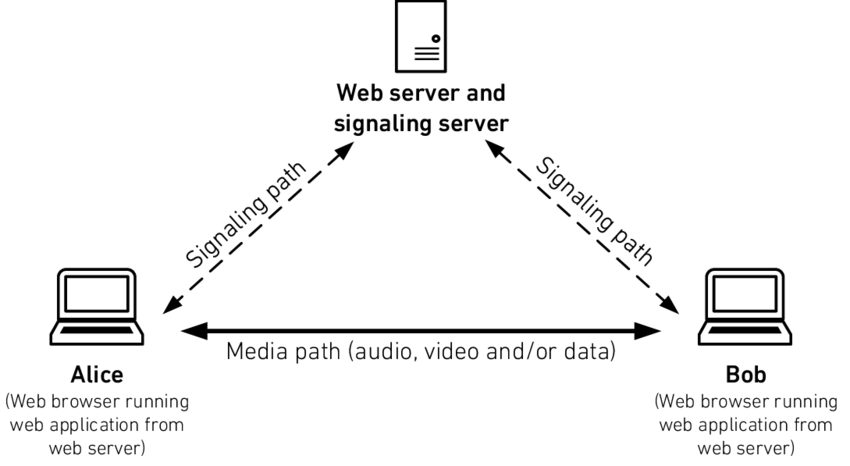
\includegraphics[width=0.7\textwidth]{img/triangolo.PNG}
 		\caption{Modello triangolare \cite{59}.}
 	\end{figure}
 	$\\$
 	\newpage
 	Esiste anche un altro modello, ispirato a quello trapezoidale di SIP (Session Initial Protocol), dove i client eseguono un'applicazione web da server diversi. Questo modello viene utilizzato meno perché rispetto a quello a triangolo consente agli sviluppatori Web una minore flessibilità nella gestione delle connessioni degli utenti \cite{12}.$\\$
 	\begin{figure}[h!]
 		\centering
 		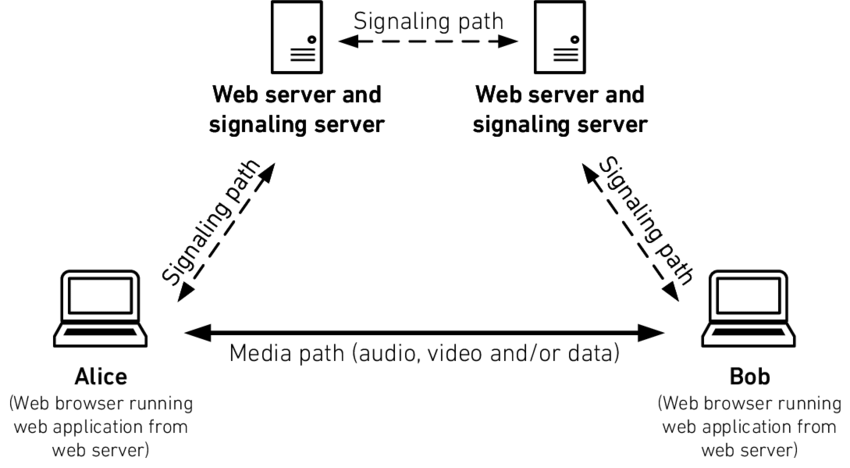
\includegraphics[width=0.7\textwidth]{img/trapezio.PNG}
 		\caption{Modello trapezoidale \cite{60}.}
 	\end{figure}
 	$\\$ $\\$ $\\$
 	
 	\newpage
 	\section{API}
 	Nel contesto di WebRTC, le API rappresentano la componente principale per il funzionamento di questa tecnologia, sia per quanto riguarda la connessione tra utenti, sia per quanto riguarda il riconoscimento di dispositivi video ed audio utilizzati. $\\$ 
 	Ma cos'è un API? Un Application Programming Interface è un'interfaccia tra due o più software che permette di farli comunicare tra loro. Un documento o uno standard che descrive come creare o utilizzare tale connessione o interfaccia è chiamato API specification. Si dice che un sistema informatico che soddisfa questo standard implementi un'API. Il termine API può riferirsi alla specifica o all'implementazione. un'API è simile a una GUI (Graphical User Interface) con una grande differenza: un'API aiuta gli sviluppatori di software ad accedere agli strumenti web mentre una GUI aiuta a rendere un programma più facile da capire per gli utenti \cite{13}. $\\$ 
 	Un'API è spesso composta da diverse parti che fungono da strumenti o servizi disponibili per il programmatore. Si dice che un programma o un programmatore che utilizza una di queste parti chiami quella parte dell'API. Le chiamate che costituiscono l'API sono anche note come subroutine, metodi, richieste o endpoint. Un'API può essere creata su misura per una particolare coppia di sistemi o può essere uno standard condiviso che consente l'interoperabilità tra molti sistemi \cite{14}. $\\$
 	L'obbiettivo di un API è quello di semplificare la programmazione, nascondendo i dettagli interni di come funziona un sistema, esponendo solo quelle parti che un programmatore troverà utili e mantenendole coerenti anche se i dettagli interni in seguito cambiano; per esempio, un'API per l'input/output di file potrebbe fornire allo sviluppatore una funzione che copia un file da una posizione a un'altra senza richiedere che lo sviluppatore comprenda le operazioni del file system che si verificano dietro le quinte. $\\$
 	L'utilizzo di API può essere fatto in diversi scenari, come nei linguaggi di programmazione, librerie software, sistemi operativi e hardware per computer. Nonostante la loro nascita ed inizio utilizzo siano datati (la loro origine risale agli anni '40, ma inizieranno ad essere utilizzate solo negli anni '60), ancora oggi sono molto impiegate e di vitale importanza per il funzionamento di programmi che le utilizzano (come WebRTC) \cite{14}.$\\$
 	\begin{figure}[h!]
 		\centering
 		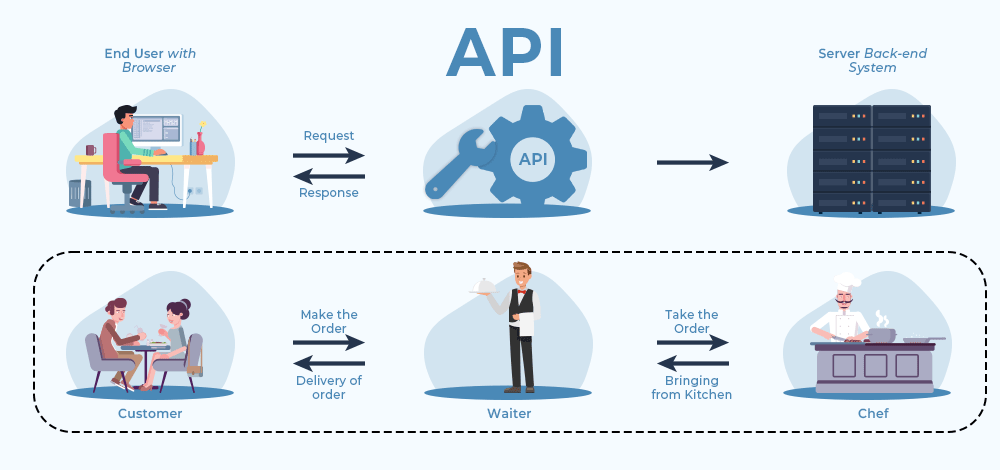
\includegraphics[width=0.7\textwidth]{img/API.PNG}
 		\caption{funzionamento di un API \cite{61}.}
 	\end{figure}
 	\newpage
 	La quantità di API esistenti e il loro funzionamento diverso ha portato ad una suddivisione di queste in diverse categorie; La maggior parte delle API utilizzate per il funzionamento di WebRTC appartengono alla categoria delle Web API, che consente la comunicazione tra computer collegati ad Internet ed accessibili utilizzando il protocollo HTTP \cite{15}. $\\$
 	Come già detto, le API rappresentano la componente principale per il funzionamento di WebRTC, e questa tecnologia ne utilizza in gran numero, ma le fondamentali sono: RTCPeerConnection, RTCDataChannel e MediaStream.
 
 	$\\$
 	\subsection{RTCPeerConnection}
 	L'interfaccia RTCPeerConnection rappresenta la componente fondamentale per impostare una connessione peer tra due o più utenti. L'attività principale dell'oggetto RTCPeerConnection è fornire metodi per connettersi ad altri utenti, mantenere e monitorare la connessione e chiuderla quando non è più necessaria. Gestisce anche una connessione UDP con un altro utente \cite{16}. $\\$ RTCpeerConnection è un oggetto Javascript, che può essere creato nel seguente modo:$\\$
 	\begin{lstlisting}
 		var pc = new RTCPeerConnection(config);
 	\end{lstlisting}
 	$\\$
 	il nuovo oggetto RTCPeerConnection rappresenta una connessione tra un dispositivo locale e un peer remoto. Al costruttore, come in questo caso, può essere passato il parametro config, un oggetto che fornisce opzioni per configurare la nuova connessione.$\\$
 	Tra i tanti metodi che RTCPeerConnection possiede ci sono \cite{16}:
 	\begin{itemize}
 		\item createOffer: crea una offerta SDP con lo scopo di iniziare una nuova connessione WebRTC con un altro utente.
 		\item createAnswer: crea una risposta SDP a un'offerta ricevuta da un peer remoto durante la negoziazione offerta/risposta di una connessione WebRTC.
 		\item addStream: aggiunge un MediaStream come sorgente locale di audio o video. Questo metodo è deprecato e obsoleto, quindi potrebbe non funzionare su alcuni browser; per questo motivo è meglio utilizzare addTrack() una volta per ogni traccia che si desideri inviare al peer remoto.
 	\end{itemize}  
 	
 	\newpage
 	\subsection{RTCDataChannel}
 	RTCDataChannel rappresenta un canale di rete che viene utilizzato per il trasferimento di dati tramite una connessione peer-to-peer bidirezionale. per questo motivo, ogni canale dati è associato a un RTCPeerConnection e ogni connessione peer può avere fino a un massimo di 65.534 canali dati (il limite effettivo può variare da browser a browser). Come vedremo successivamente, i canali dati utilizzano il protocollo SCTP, che permette di stabilire una connessione TCP o UDP in base al tipo di traffico che si desidera spedire.$\\$ 	
 	Per creare un canale dati e chiedere ad un utente di unirsi, si deve utilizzare il metodo createDataChannel() di RTCPeerConnection. Questo crea un nuovo canale connesso al peer remoto sul quale è possibile trasferire qualsiasi tipo di dati (a differenza di media stream, dove si può solo trasmettere video ed immagini). createDataChannel() ha due parametri, label (campo obbligatorio) che corrisponde al nome del canale dati, e options (campo opzionale), il parametro che fornisce delle opzioni di configurazione per il canale. l'utente invitato a scambiare dati riceve un evento datachannel per informarlo che il canale dati è stato aggiunto alla connessione \cite{17}.$\\$
 	Un esempio di codice di createDataChannel potrebbe essere il seguente:$\\$
 	\begin{lstlisting}
 	[code]
 	//establishing peer connection
 	var peerConn = new RTCPeerConnection(); 
 	//...
 	//end of establishing peer connection
 	//here we can start sending direct messages to another peer
 	var dataChannel = peerConnection.createDataChannel("myChannel", 
 	dataChannelOptions); 
 	[/code]
 	\end{lstlisting}
 	$\\$
 	\newpage
 	\subsection{MediaStream}
 	MediaStream è un API che viene messa a disposizione dai browser agli sviluppatori per accedere agli stream (insieme di tracce audio/video) tramite i dispositivi dell'utente. Questa API ha tre funzionalità principali \cite{12}:
 	\begin{itemize}
 		\item Fornisce a uno sviluppatore l'accesso a un oggetto stream.
 		\item Gestisce la selezione dei dispositivi input dell'utente nel caso in cui questo disponga di più telecamere o microfoni sul proprio dispositivo.
 		\item Fornisce un livello di sicurezza attraverso richieste di autorizzazioni all'utente, effettuate prima che un'applicazione Web possa iniziare a recuperare uno stream.
 	\end{itemize}
 	Un oggetto MediaStream si ottiene in due modi: creandolo tramite il suo costruttore oppure richiamando un metodo che lo restituisce. Il costruttore crea un nuovo oggetto MediaStream che può essere uno stream vuoto(nessun parametro), uno stream basato su un altro stream esistente passato come parametro oppure uno stream che contiene un array specifico di tracce (di tipo MediaStreamTrack). $\\$
 	il metodo più importante che crea un Mediastream è getUserMedia() di MediaDevice. Quello che fa questo metodo è richiedere l'autorizzazione all'utente per utilizzare i dispositivi di input, creando un MediaStream che contiene le tracce per i tipi di media richiesti.
 	Un Altro metodo molto utilizzato che restituisce un MediaStream è getDisplayMedia(), che, come getUserMedia(), richiede all'utente l'autorizzazione per la condivisione del suo schermo \cite{18}. 
 	\newpage
 	\subsection{altre API}
 	Oltre alle API citate, ne esistono molte altre, ognuna con il proprio compito. Alcune di queste sono \cite{19}:
 	\begin{itemize}
 		\item MediaDevice: un'API che fornisce l'accesso ai dispositivi di input multimediali collegati come fotocamere, microfoni e condivisione dello schermo.
 		\item MediaStreamTrack: rappresenta una singola traccia multimediale all'interno di uno stream; in genere si tratta di tracce audio o video, ma possono esistere anche altri tipi di tracce.
 		\item RTCDataChannelEvent: rappresenta un evento correlato ad un RTCDataChannel.
 		\item RTCIceTransport: API che fornisce informazioni sul livello di trasporto ICE utilizzato per l'invio ed il ricevimento dei dati. Viene adottata se è necessario accedere alle informazioni sullo stato della connessione.
 		\item RTCSessionDescription: Descrive un'estremità di una connessione e come è configurata.
 	\end{itemize}
 	
 	\newpage
   	\section{Protocolli}
  	La pila protocollare di WebRTC è la seguente:
  	\begin{figure}[h!]
  		\centering
  		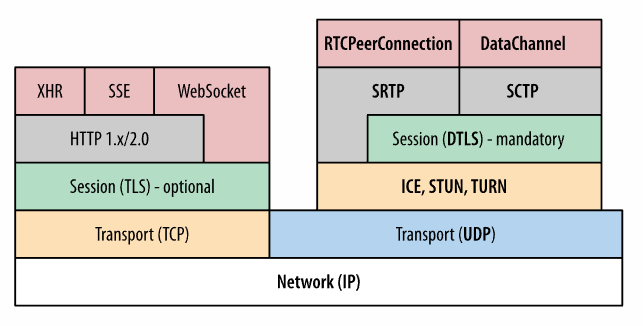
\includegraphics[width=0.7\textwidth]{img/PilaProtocollare2.jpg}
  		\caption{Pila protocollare di WebRTC \cite{62}.}
  	\end{figure}
  	$\\$ $\\$
  	\subsection{Trasporto}
  	Come si può notare, WebRTC può utilizzare sia UDP o TCP a livello di trasporto, ma, a differenza della maggior parte delle applicazioni web, WebRTC utilizza quasi sempre UDP per la spedizione di dati. Perché questo? Come già detto, TCP è più utilizzato perché è più affidabile rispetto a UDP. Questo perché nello spedire dati, TCP garantisce che \cite{20}:
  	\begin{itemize}
  		\item Ogni dato spedito viene marcato come consegnato.
  		\item Ogni dato che non arriva al mittente viene rispedito e la spedizione di messaggi viene temporaneamente disattivata.
  		\item Ogni dato è unico senza duplicati dalla parte del mittente.
  		\item Tutti i dati spediti arrivino in ordine.
  	\end{itemize}
  	per questi motivi TCP è adottato dalle maggior parte delle applicazioni Web. Nel richiedere una pagina HTLM, per esempio, tutti i dati devono arrivare nel corretto ordine. Ma questa applicazione non è adatta a tutti gli scenari; infatti le applicazioni per la trasmissione di video e audio richiedono una connessione più veloce. Ed è per questo che UDP è utilizzato. Questo protocollo, a differenza di TCP, non garantisce il corretto ordine dei dati spediti e non da informazione sullo stato di ogni pacchetto, ma la velocità di spedizione di dati è nettamente superiore. Inoltre, nelle applicazioni di streaming video o audio dove vengono spediti un determinato numero di frame al secondo, è più importante l'invio dell'ultimo frame rispetto all'invio di ogni singolo frame. Quindi è possibile perdere qualche frame senza che l'utente se ne accorga perché li rimpiazzerà con ciò che vede. Questo è un altro motivo per cui UDP è più utilizzato \cite{12}. $\\$ L'unico caso in cui viene utilizzato TCP nelle applicazioni WebRTC è quello in cui UDP non è disponibile, per esempio quando è bloccato dal firewall \cite{21}.
  	\newpage
  	\subsection{Instradamento}
  	Quando si vuole effettuare una connessione tra due utenti è necessario creare una "strada" tra questi due. Questo lavoro può essere complesso perché è probabile che le reti dei due utenti abbiano diversi livelli di controllo legati alla sicurezza. Esistono però tecnologie utilizzate per trovare un percorso chiaro verso un altro utente, tra cui \cite{12}:
  	\begin{itemize}
  		\item STUN (Session Traversal Utilities for NAT).
  		\item TURN (Traversal Using Relays around NAT).
  	\end{itemize}
  	STUN è un insieme standardizzato di metodi utilizzato per l'attraversamento di gateway NAT (Appendice B), permettendo agli host di conoscere i propri indirizzi IP che servono, nel contesto di WebRTC, per effettuare comunicazioni peer to peer attraverso Internet \cite{22}. Per farlo, un host invia una richiesta al server STUN per ottenere l'IP pubblico e le informazioni sulle porte; di conseguenza il server STUN recupera tali informazioni:
  	\begin{figure}[h!]
			\centering
			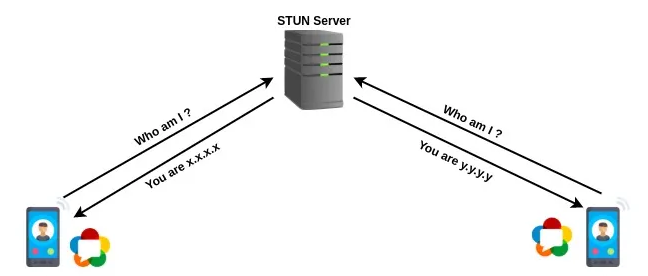
\includegraphics[width=0.7\textwidth]{img/stun-server3.png}
			\caption{Funzionamento di STUN \cite{63}.}
  	\end{figure}
  	$\\$ 
  	A volte, però, STUN potrebbe non essere utilizzabile, come nel caso di NAT simmetrici che, a causa delle loro restrizioni, non permettono a STUN di funzionare. In questi casi viene utilizzato TURN.$\\$
  	TURN consente a un server di inoltrare pacchetti di dati (media nel caso di WebRTC) tra peer attraverso un server TURN intermedio. I peer possono instradare i media al server TURN che li trasmetterà continuamente all'altro peer. Dal momento che il server inoltra tutti i media in continuazione, questa procedura richiede uno sforzo piuttosto costoso. Questo è il motivo per cui TURN viene utilizzato quando non sono possibili connessioni dirette e non ci sono altre alternative \cite{23}.
  	\begin{figure}[h!]
  		\centering
  		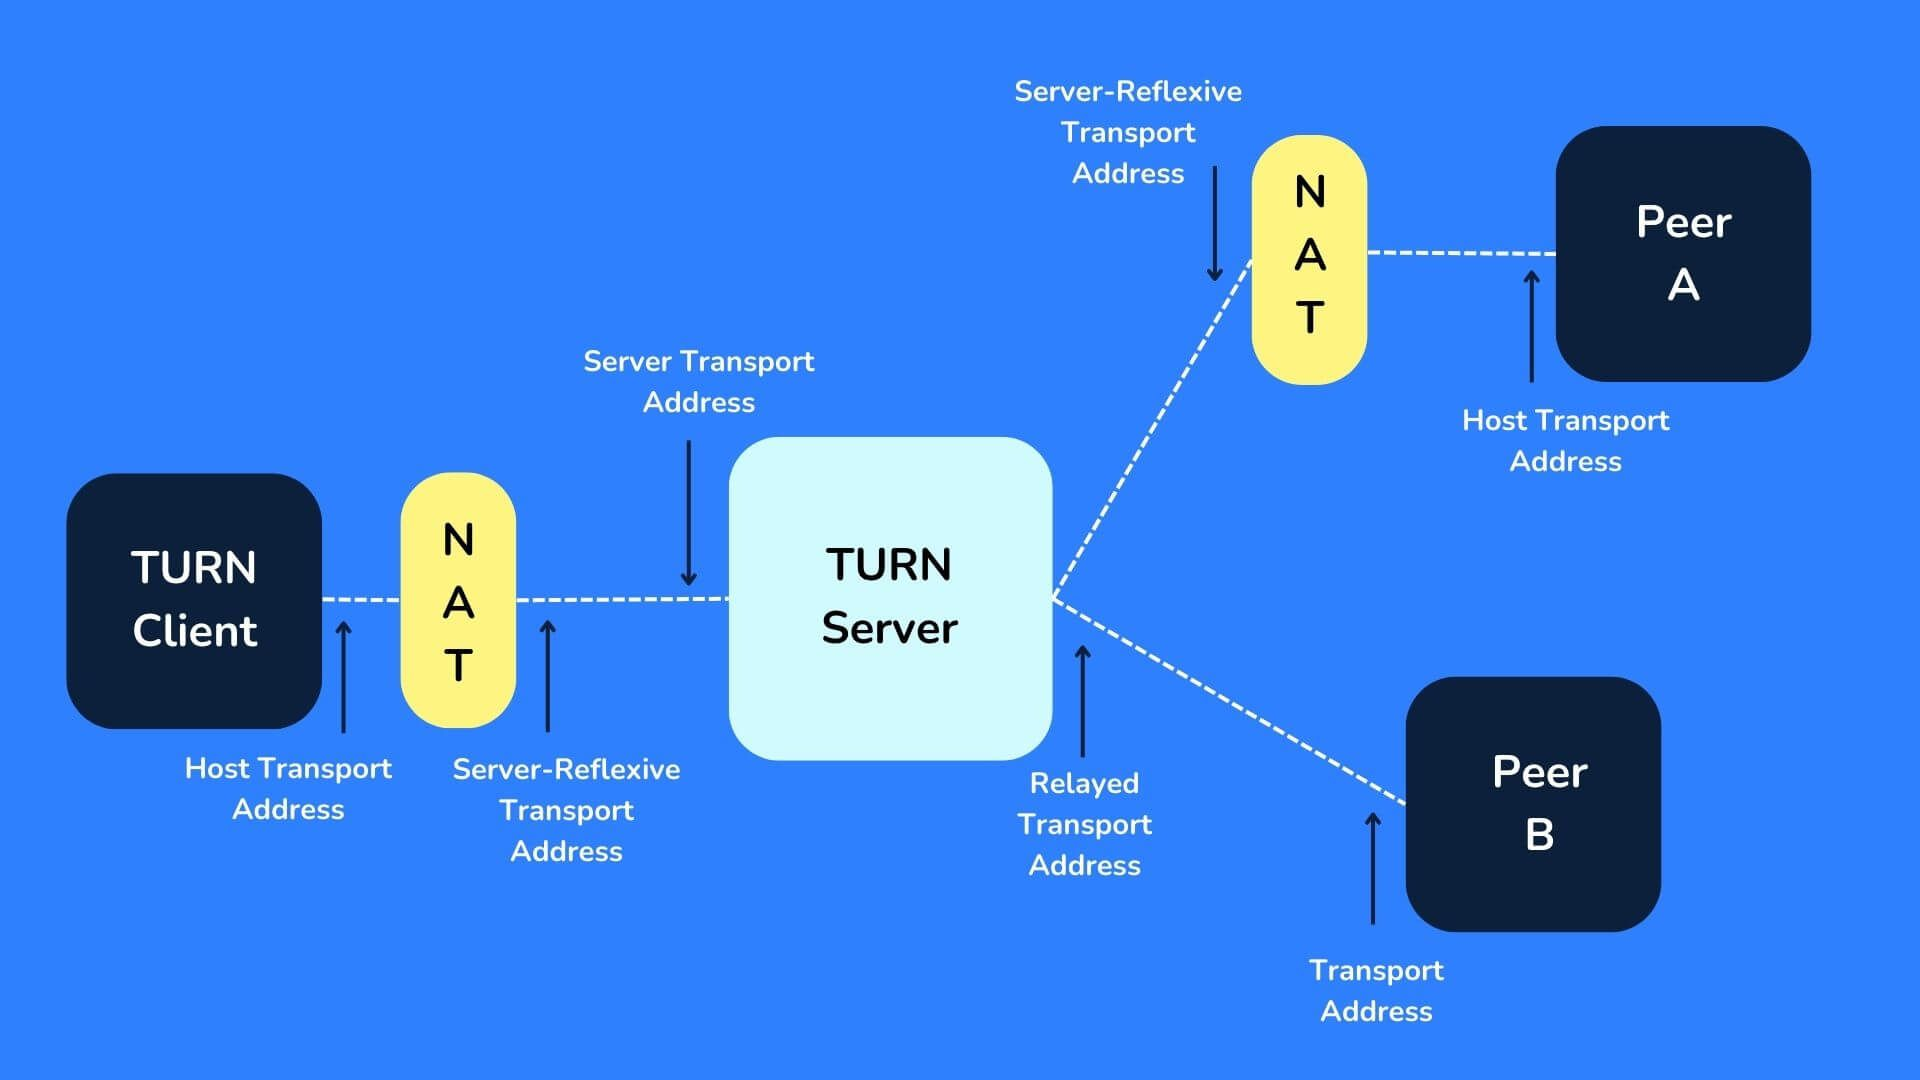
\includegraphics[width=0.6\textwidth]{img/turn.jpg}
  		\caption{Funzionamento di TURN \cite{64}.}
  	\end{figure}
  	\newpage
  	Per trovare il miglior percorso, WebRTC utilizza ICE (Interactive Connectivity Establishment), una tecnologia che permette di utilizzare STUN e TURN assieme. ICE utilizza queste due tecnologie per creare la migliore connessione peer to peer tra gli utenti, trovando e verificando in ordine una serie di indirizzi che funzionino per tutti. Al suo avvio, ICE non conosce la rete di ciascun utente, quindi la prima cosa che fa è attraversare una serie di fasi in modo incrementale per scoprire come è configurata la rete di ciascun client, utilizzando un diverso insieme di tecnologie.$\\$ 
  	STUN e TURN sono usati per trovare ogni candidato ICE, un elemento creato dai peer che descrive il routing e i protocolli necessari affinché WebRTC sia in grado di comunicare con un dispositivo remoto. ICE utilizzerà il server STUN per trovare un IP esterno. Se la connessione fallisce, tenterà di utilizzare il server TURN. Quando si avvia una connessione peer WebRTC, in genere viene proposto un numero di candidati da ciascuna estremità della connessione, fino a quando essi non concordano reciprocamente su quello che ritengono più efficiente. WebRTC utilizza quindi i dettagli di quel candidato per avviare la connessione. \cite{24}. 
  	\begin{figure}[h!]
  		\centering
  		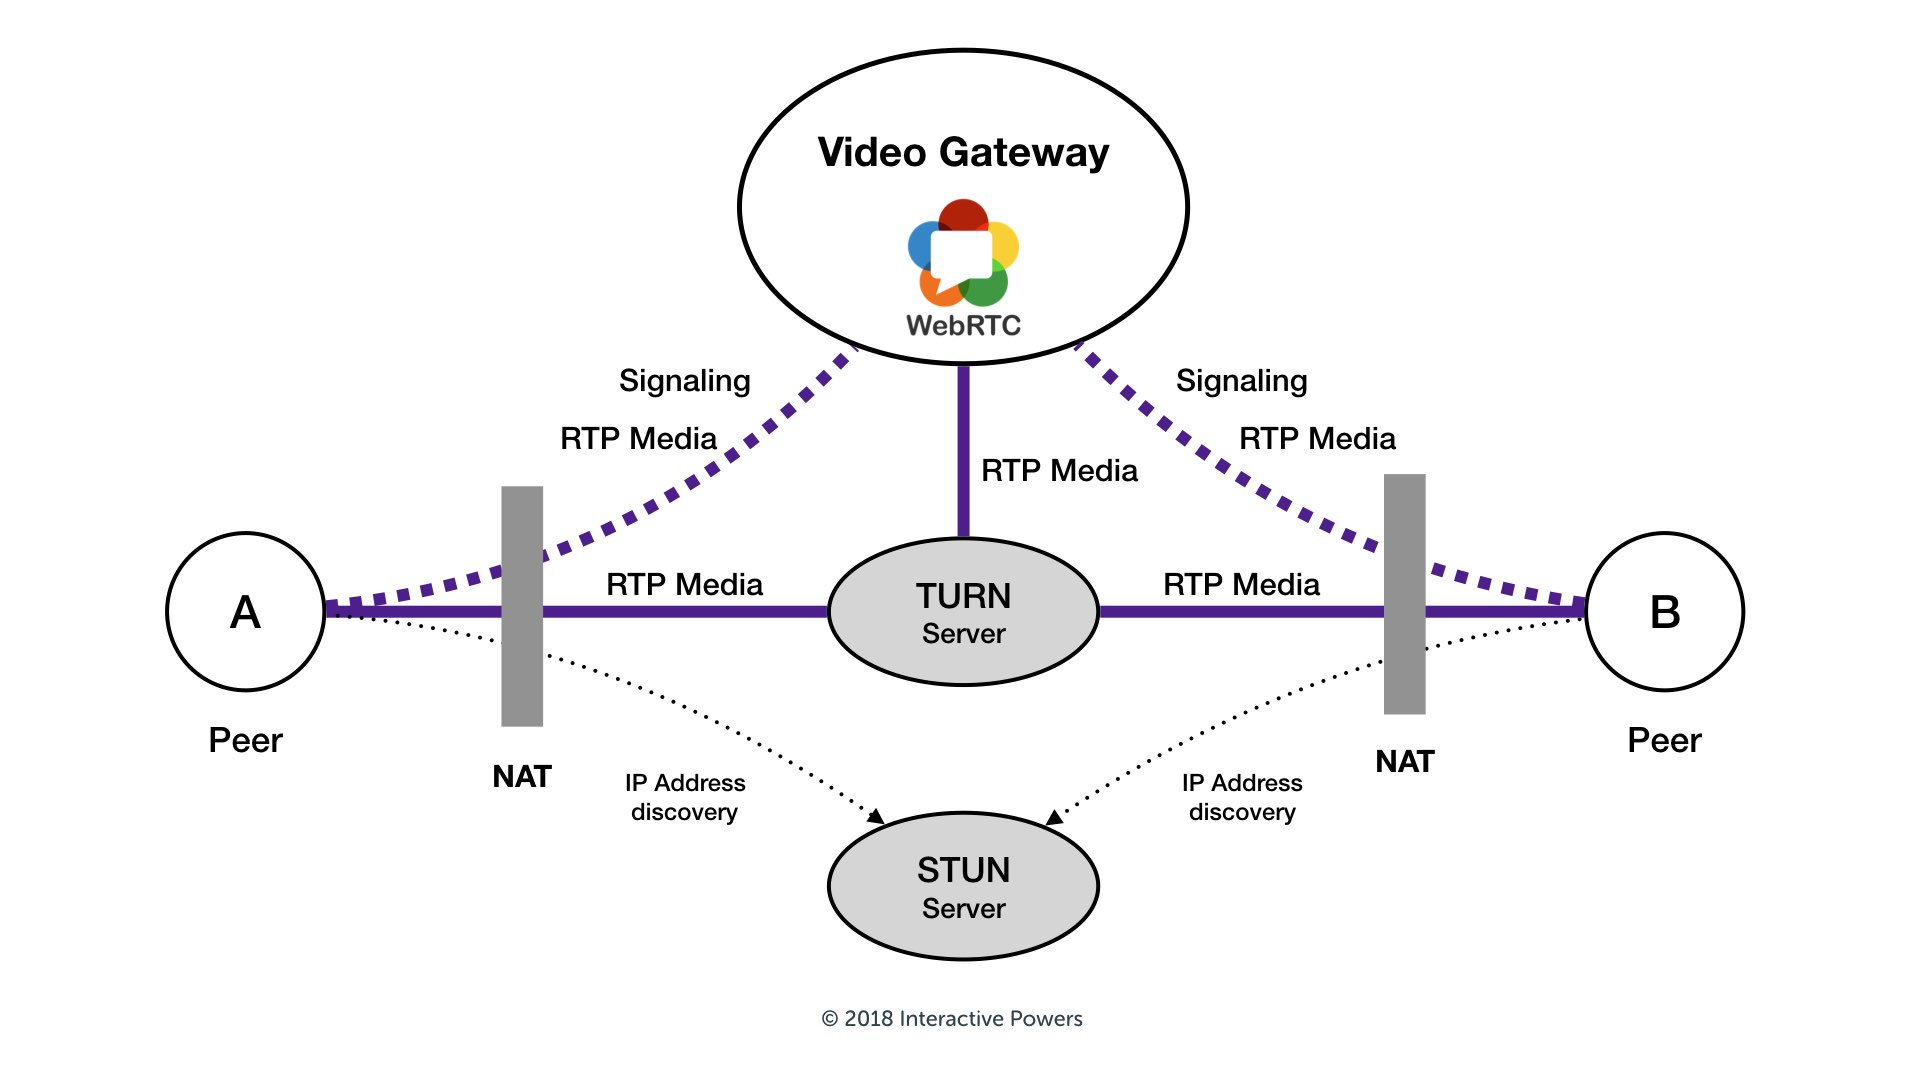
\includegraphics[width=0.9\textwidth]{img/ICE.jpeg}
  		\caption{Funzionamento di ICE \cite{62}.}
  	\end{figure} 
  	\newpage
  	
  	\subsection{altri protocolli}
  	SDP (Session Description Protocol) è uno standard per descrivere informazioni come il tipo di dati inviati, il protocollo di trasferimento utilizzato, l'indirizzo IP, la porta degli utenti e tutte le altre informazioni che permettono ai peer di capirsi una volta che i dati vengono trasferiti. Quindi SDP è un protocollo che descrive il formato di dati che i peer si scambiano per descrivere la connessione. WebRTC utilizza questo protocollo per negoziare i parametri della sessione durante la fase di signaling \cite{25}.$\\$
  	SCTP (Stream Control Transmission Protocol) è un protocollo di trasporto che viene utilizzato per inviare rapidamente dati attraverso i Data Channel. Quando un applicazione WebRTC utilizza un canale dati in base alle esigenze può utilizzare UDP o TCP. Per questo motivo SCTP viene utilizzato da WebRTC, perché ha caratteristiche che soddisfano sia UDP che TCP, come la protezione del livello di trasporto effettuata da DTLS, la possibilità, durante la spedizione, di poter scomporre e riassemblare i dati dalla parte del destinatario, poter disattivare l'affidabilità e la spedizione ordinata, garantendo la latenza necessaria per i sistemi in tempo reale \cite{12}. $\\$
  	WebRTC utilizza RTP (Real time protocol) per scambiare contenuti multimediali crittografati tramite SRTP. RTP è un protocollo che fornisce gli strumenti necessari per implementare lo streaming in tempo reale. La cosa più importante di questo protocollo è che offre flessibilità allo sviluppatore, consentendogli di gestire la latenza, la perdita di pacchetti e la congestione \cite{26}. 
  	\newpage
  	\section{Funzionamento}
  	\subsection{Signaling}
 	Prima di poter iniziare una comunicazione tramite WebRTC, gli utenti interessati devono effettuare uno scambio di informazioni; questo processo si chiama signaling. Durante questa fase, lo scambio di informazioni determina i protocolli di comunicazione, i canali, i codec, i formati multimediali e il metodo di trasferimento dei dati, nonché qualsiasi informazione di instradamento richiesta. Nelle specifiche di WebRTC non è descritto uno standard da seguire per effettuare il signaling e qualsiasi utente può effettuarlo in modo differente. Un esempio di signaling potrebbe avvenire in questo modo \cite{12}:
 	\begin{itemize}
 		\item Viene creata una lista dei potenziali candidati alla connessione peer.
 		\item un utente sceglie un'altra persona con cui stabilire una connessione. 
 		\item Il signaling layer avverte l'altro utente che qualcuno sta provando a connettersi a lui. A questo punto può accettare o rifiutare.
 		\item Se accetta, l'utente chiamante viene notificato.
 		\item Quest'ultimo inizializza una RTCPeerConnection con l'altro utente.
 		\item Entrambi gli utenti si scambiano informazioni riguardanti software e hardware attraverso il signaling server.
 		\item Entrambi si scambiano informazioni sulla posizione.
 		\item Fatto tutto ciò la connessione può iniziare, a meno che non fallisca.
 	\end{itemize}
 	\begin{figure}[h!]
 		\centering
 		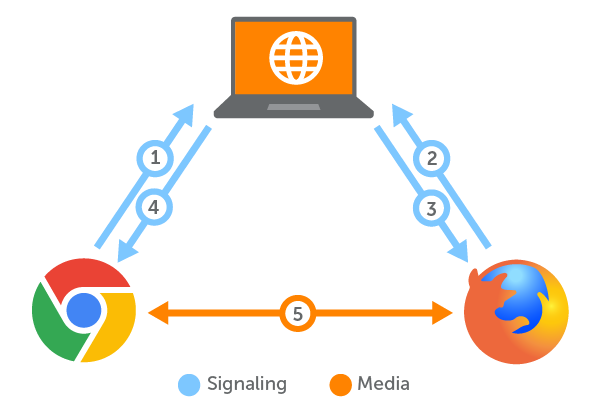
\includegraphics[width=0.6\textwidth]{img/Signaling.png}
 		\caption{Esempio di Signaling \cite{65}.}
 	\end{figure}
 	\newpage
 	\subsection{Signaling con WebSocket}
 	Un altro esempio di signaling può essere fatto con uno dei meccanismi più utilizzati per effettuare questo processo: il protocollo WebSocket, che consente ai peer di scambiare informazioni sulla connessione in tempo reale tramite un server WebSocket. Per realizzare un servizio di questo tipo è necessario stabilire una connessione bidirezionale WebSocket tra uno o più browser e un server. Successivamente si passa all'integrazione del servizio WebSocket nel server HTTP, aprendo la porta WebSocket e mettendolo in ascolto. Nel browser, è necessario creare un oggetto WebSocket in base all'indirizzo e alla porta del server. La connessione WebSocket verrà creata dopo l'handshake. Effettuati tutti questi passaggi, il browser e il server sono in grado di scambiarsi informazioni \cite{27}: $\\$
 	\begin{figure}[h!]
 		\centering
 		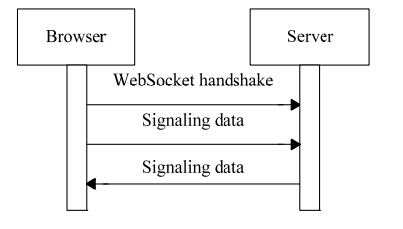
\includegraphics[width=0.5\textwidth]{img/WebSocket.png}
 		\caption{Esempio di Signaling con Websocket.}
 	\end{figure}
 	$\\$
 	Una volta stabilita la connessione tra browser e server segue l'identificazione tra utenti, necessaria per lo scambio di informazioni di negoziazione. Per farlo possono essere utilizzate le Rooms di socket.io, un meccanismo che in questo contesto ha lo scopo di ottenere l'identificazione tra gli utenti. Il processo di identificazione tra due peer è il seguente [27]:
 	\begin{itemize}
 		\item Un utente A visita l'indirizzo di una Room e stabilisce una connessione WebSocket con il server. 
 		\item Successivamente, il browser spedisce un messaggio (join\_in) al server, il cui contenuto descrive l'identificazione della room.
 		\item Una volta ricevuto il messaggio, il server verifica se esiste una room con lo stesso nome del messaggio di A. In caso negativo, ne crea una nuova.
 		\item Un utente B che vuole comunicare con A si collega all'indirizzo della stessa room a cui si è collegato l'utente A ed effettua lo stesso procedimento visto al primo punto.
 		\item ottenuto il messaggio di B, il server genera dei SocketID diversi per ogni utente e li spedisce in broadcast ad ogni peer.
 	\end{itemize} 
 	Questi ID servono per identificare ogni utente. Se A desidera negoziare i parametri per una connessione WebRTC con B, deve solo inviare il messaggio di negoziazione e il socketID dell'utente B al server. Questo selezionerà l'utente B tramite socketID e inoltrerà il messaggio dall'utente A. La risposta dall'utente B all'utente A segue la stessa procedura.
 	\newpage
 	\subsection{Connessione}
 	Una volta scambiati i parametri per stabilire la connessione, intervengono le API.$\\$
 	La prima che viene utilizzata è MediaStream che con getUserMedia richiede l'autorizzazione per accedere agli stream audio e video dell'utente tramite microfono e webcam, permettendo di selezionare quali input utilizzare, nel caso l'utente ne abbia più di uno.   $\\$
 	Dopo aver ottenuto un flusso multimediale tramite l'API getUserMedia, il passaggio successivo di un'app WebRTC è quello di trasmettere i dati in tempo reale a un altro browser. Prima però è necessario stabilire una connessione tra due (o più) utenti. Questo è il compito principale di RTCPeerConnection. Supponiamo che due utenti vogliano comunicare tra loro; per farlo, l'utente chiamante crea un oggetto RTCPeerConnection per stabilire la connessione e successivamente viene creata un'offerta ed estesa all'altro browser con il metodo createOffer. Questa offerta enumera i potenziali codec, i metodi di crittografia, i possibili ICE e altre informazioni iniziali disponibili per una sessione WebRTC. Questo processo utilizza SDP. Dopo che questa descrizione è stata generata, viene inviata al peer con la quale si vuole comunicare che, a sua volta, genera una risposta SDP con il metodo createAnswer (la risposta contiene informazioni su qualsiasi supporto già collegato alla sessione, codec e opzioni supportate dal browser e qualsiasi candidato ICE già raccolto) e la spedisce al chiamante. Quando la risposta arriva a quest'ultimo, la connessione viene stabilita \cite{16}.$\\$
 	L'ultima operazione da effettuare è trasmettere dati in tempo reale. Questo compito è effettuato da RTCDataChannel. Grazie a questa API è possibile creare canali dati associati a una RTCPeerConnection semplicemente richiamando il metodo createDataChannel(). Fatto ciò è possibile spedire messaggi tramite il protocollo SCTP che saranno crittografati con DTLS \cite{28}.
	\begin{figure}[h!]
		\centering
		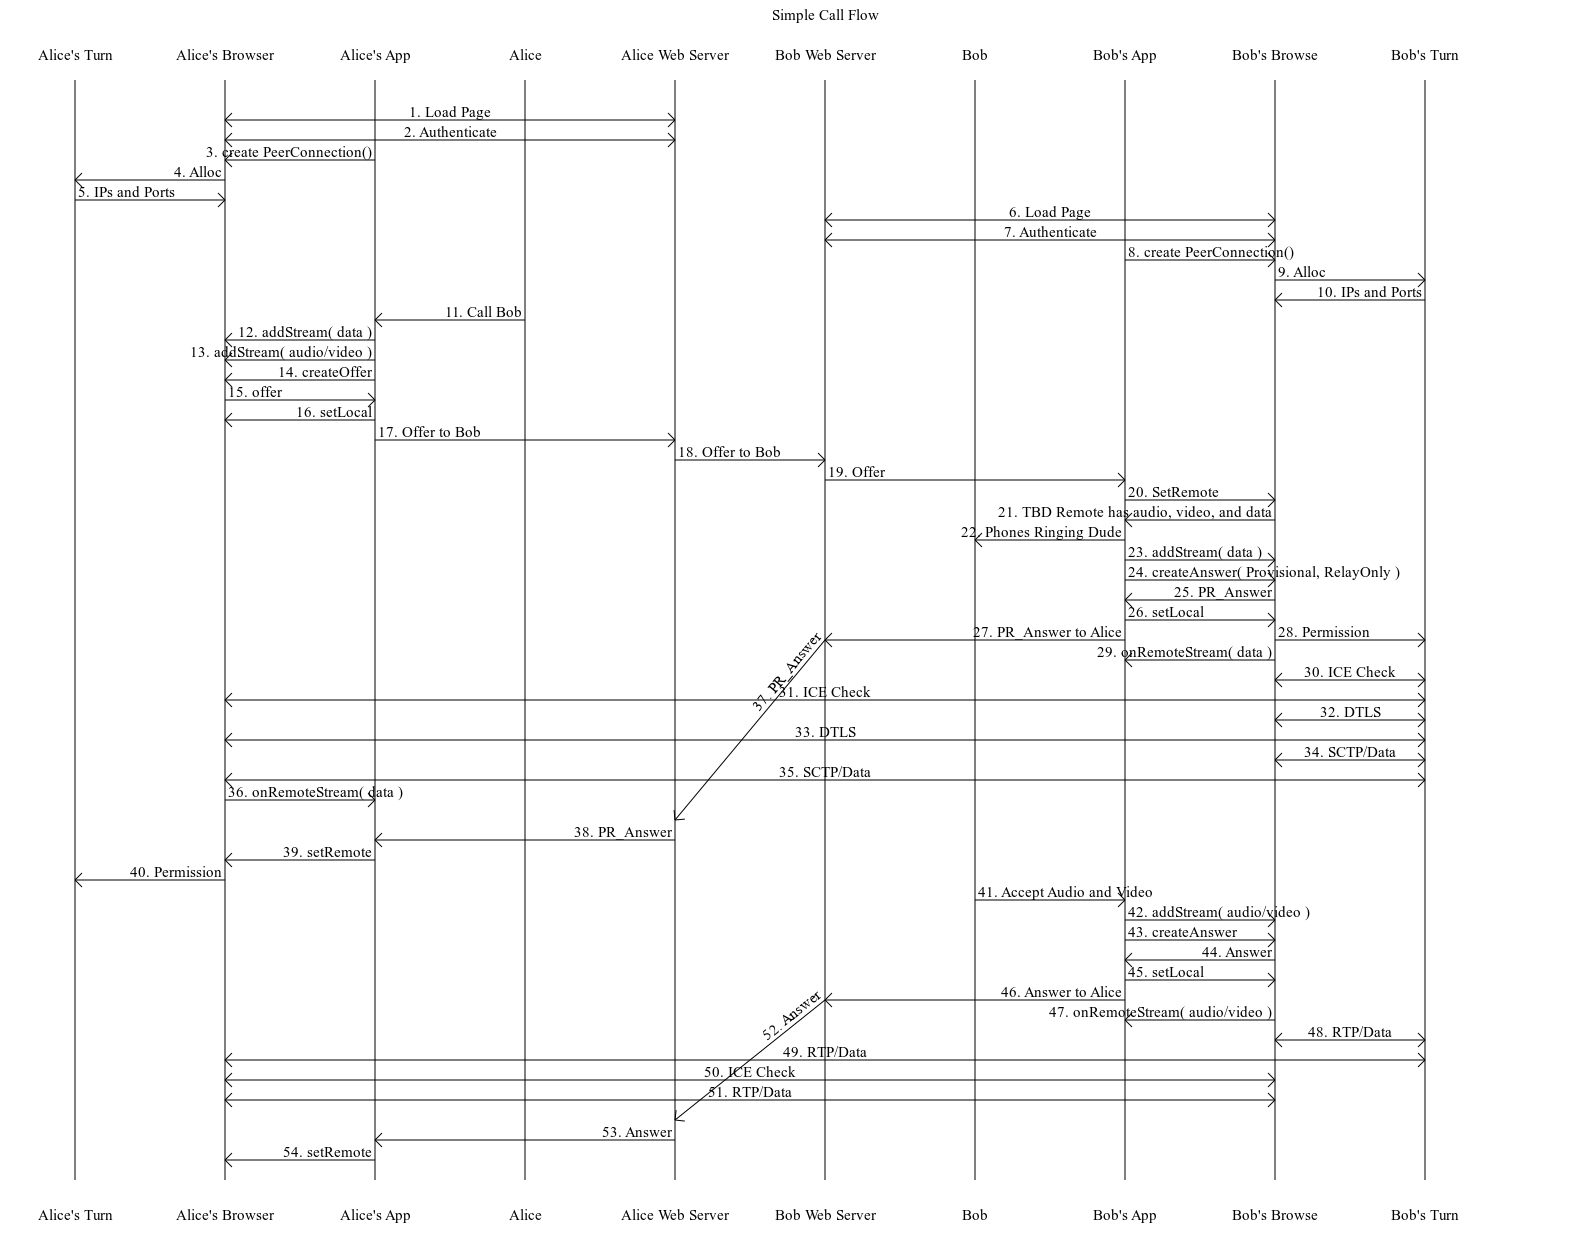
\includegraphics[width=0.9\textwidth]{img/WebRTCCallFlow.png}
		\caption{Un possibile esempio di chiamata tra due utenti \cite{66}.}
	\end{figure} 	
 	\newpage
 	\section{Supporto}
 	Alla fine del 2018 tutti i principali browser e sistemi operativi per dispositivi mobili
 	hanno cominciato a supportare WebRTC. Nonostante ciò è possibile che alcune operazioni possano funzionare erroneamente o non funzionare completamente. Un esempio è l'utilizzo di Microsoft Teams su Firefox: l'app funziona, ma non completamente, perché su questo browser non sono disponibili alcune funzioni che su Chrome, per esempio, sono supportate \cite{29}.
 	Di seguito si analizzerà il supporto browser e mobile di WebRTC.
 	\subsection{Browser}
 	Il primo browser che ha supportato WebRTC è ovviamente Chrome (in quanto sono entrambi prodotti da Google) con la versione 23 rilasciata nel novembre del 2012. Solo su Chrome, inoltre, è possibile visualizzare alcune informazioni dei flussi audio e video, sia inviati che ricevuti, in esecuzione su una comunicazione, come i pacchetti persi, quanti bit e pacchetti vengono ricevuti o spediti al secondo \cite{30}.$\\$ 
 	Nel giro di un anno, anche Firefox e Opera hanno rilasciato le prime versioni con supporto WebRTC. Nello stesso periodo gli sviluppatori di Chrome e Firefox iniziarono a lavorare assieme per risolvere i possibili problemi che non permettevano la comunicazione tramite questi due browser \cite{12}. $\\$
 	Il supporto su Safari arrivò molto più tardi, con Safari 11 nel 2017. Questo ritardo è dato da due possibili motivazioni: la prima è la natura di Apple, che rende complesso lo sviluppo e l'uso di tecnologie non prodotte da Apple stessa; la stessa cosa si verifica su iOS. La seconda motivazione era la minaccia economica che costituiva WebRTC per le app di comunicazione real-time sull'Apple strore, come Facetime \cite{31}.  $\\$
 	Come si nota in figura, l'unico browser che non supporta WebRTC è Internet Explorer in quanto nel corso degli anni è stato sempre meno utilizzato fino a non essere più supportato da Microsoft stessa nel febbraio del 2022, lasciando il posto ad Edge, che ha iniziato a supportate WebRTC nel 2020.
 	\begin{figure}[h!]
 		\centering
 		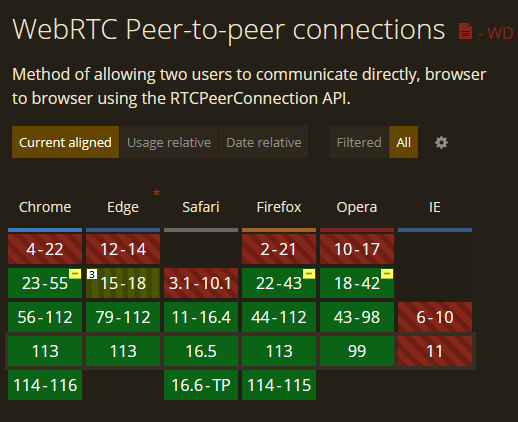
\includegraphics[width=0.6\textwidth]{img/BrowserS.png}
 		\caption{Supporto dell'API RTCPeerConnection su Browser \cite{30}.}
 	\end{figure} 	
 	\newpage
 	\subsection{Mobile}
 	Quando si parla di smartphone il supporto per WebRTC è molto più complesso da realizzare rispetto a quello su computer. Per quest'ultimi abbiamo visto che per comunicare è necessario utilizzare un browser che supporti WebRTC. Su smartphone invece anche il sistema operativo deve supportare questa tecnologia, motivo per il quale l'utilizzo di WebRTC su mobile è tardato.$\\$
 	Nel 2014, Google ha rilasciato Android 5 (conosciuto anche come Lollipop), la prima versione che supporta le tre componenti principali di WebRTC: RTCPeerConnection, MediaStream e RTCDataChannel. I browser per mobile che supportano meglio WebRTC son Chrome, Firefox e Opera [30].   $\\$
 	Il supporto su iOS è arrivato con iOS 11 nel 2017, assieme a safari, ma nonostante WebRTC sia supportato da diversi anni, è stato più volte segnalata la presenza di numerosi bug che rendono quasi inutilizzabile questa tecnologia su dispositivi iOS \cite{32}.
 	\begin{figure}[h!]
 		\centering
 		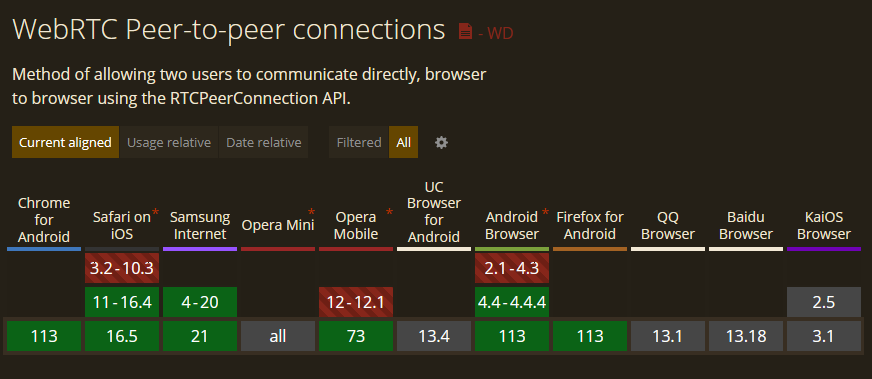
\includegraphics[width=0.7\textwidth]{img/MobileS.png}
 		\caption{Supporto dell'API RTCPeerConnection su Mobile \cite{30}.}
 	\end{figure} 	
 	\newpage
 	\section{Sicurezza}
 	WebRTC utilizza due protocolli per la sicurezza, DTLS (Datagram Transport Layer Security) e SRTP (Secure Real-time Transport Protocol).$\\$
 	DTLS è un protocollo di comunicazione che fornisce sicurezza alle applicazioni basate su datagrammi (come UDP e SCTP) consentendo agli utenti di comunicare tra loro prevenendo l'intercettazione, la manomissione o la contraffazione dei messaggi. L'obbiettivo di DTLS è quello di realizzare TLS (appendice E) per datagrammi. Il trasporto di datagrammi non richiede né fornisce una consegna affidabile o ordinata dei dati. Il protocollo DTLS conserva questa proprietà per i dati dell'applicazione. Per poter comunicare, Client e server DTLS devono concordare una cifratura e le chiavi. Questi valori vengono determinati eseguendo un handshake DTLS, che è per gran parte uguale a quello TLS. In questo processo, il client inizia la comunicazione con il server inviando un messaggio "Hello". A questo il server risponde inviando al client il proprio certificato SSL che contiene la sua chiave pubblica. Il client verifica il certificato e, una volta estratta la chiave pubblica, la utilizza per criptarerne una nuova, la chiave pre-master e la spedisce al server. Quando quest'ultimo la decritta, sia client che server la utilizzano per creare la chiave privata comune. Il client, a questo punto, spedisce un messaggio criptato con la chiave segreta appena creata al server. La stessa cosa fa ques'ultimo, determinando la fine dell'handshake DTLS \cite{33}.$\\$
 	SRTP è un protocollo utilizzato per i pacchetti RTP, destinato a fornire crittografia, autenticazione e integrità dei messaggi e protezione dagli attacchi ai dati RTP, in applicazioni sia unicast che multicast. Per avviare una sessione SRTP è necessario specificare le chiavi e la cifratura. Tutta la configurazione viene eseguita durante l'handshake DTLS poiché SRTP non ha una fase di handshake. La generazioni di chiavi viene fatta da una Key Derivation Function definita da SRTP. Quando viene creata una sessione SRTP, gli input vengono eseguiti attraverso questa funzione per generare le chiavi per il cifrario SRTP \cite{33}. $\\$
 	\begin{figure}[h!]
 		\centering
 		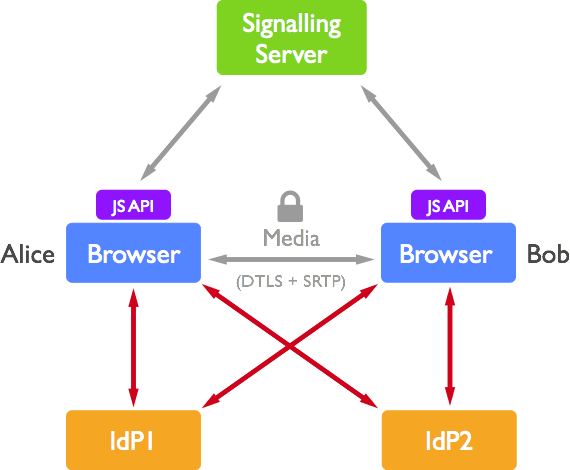
\includegraphics[width=0.6\textwidth]{img/DTLS.png}
 		\caption{funzionamento DTLS e SRTP \cite{67}.}
 	\end{figure}
 	\newpage
 	\subsection{Un possibile attacco}
 	Nonostante questi protocolli, WebRTC non è esente da problemi di sicurezza. Come descritto nei capitoli precedenti, WebRTC necessita degli indirizzi IP pubblici degli utenti per poter creare una connessione fra questi. Durante, per esempio, una videochiamata tra due utenti, si può verificare una perdita dati chiamata WebRTC leak, ovvero  un browser Web espone inavvertitamente gli indirizzi IP degli utenti. L'esposizione di un indirizzo IP può causare danni gravi a un utente; un malintenzionato che riesce ad accedere alle informazioni di identificazione personale come indirizzi IP, richieste DNS e geolocalizzazione basata su IP può utilizzare questi dati per tracciare l'attività online di un individuo. Inoltre un attaccante esperto potrebbe effettuare un NAT Slipstreaming, un attacco che consente a un utente malintenzionato di accedere in remoto a qualsiasi servizio TCP/UDP associato a un sistema dietro il NAT di una vittima, aggirando il NAT/firewall di quest'ultima \cite{34}.$\\$
 	Tutti questi problemi possono essere però prevenuti tramite l'utilizzo di una VPN (Virtual Private Network), una tecnologia che consente di creare una rete privata tra due dispositivi su Internet. Tra le tante funzioni di una VPN c'è anche quella di "cambiare" l'indirizzo IP dell'utente con un indirizzo fittizio; in questo modo è possibile navigare in sicurezza, perché nel caso ci sia una WebRTC leak, l'attacante non potrà fare nulla con l'indirizzo IP della VPN \cite{35}.
 	\begin{figure}[h!]
 		\centering
 		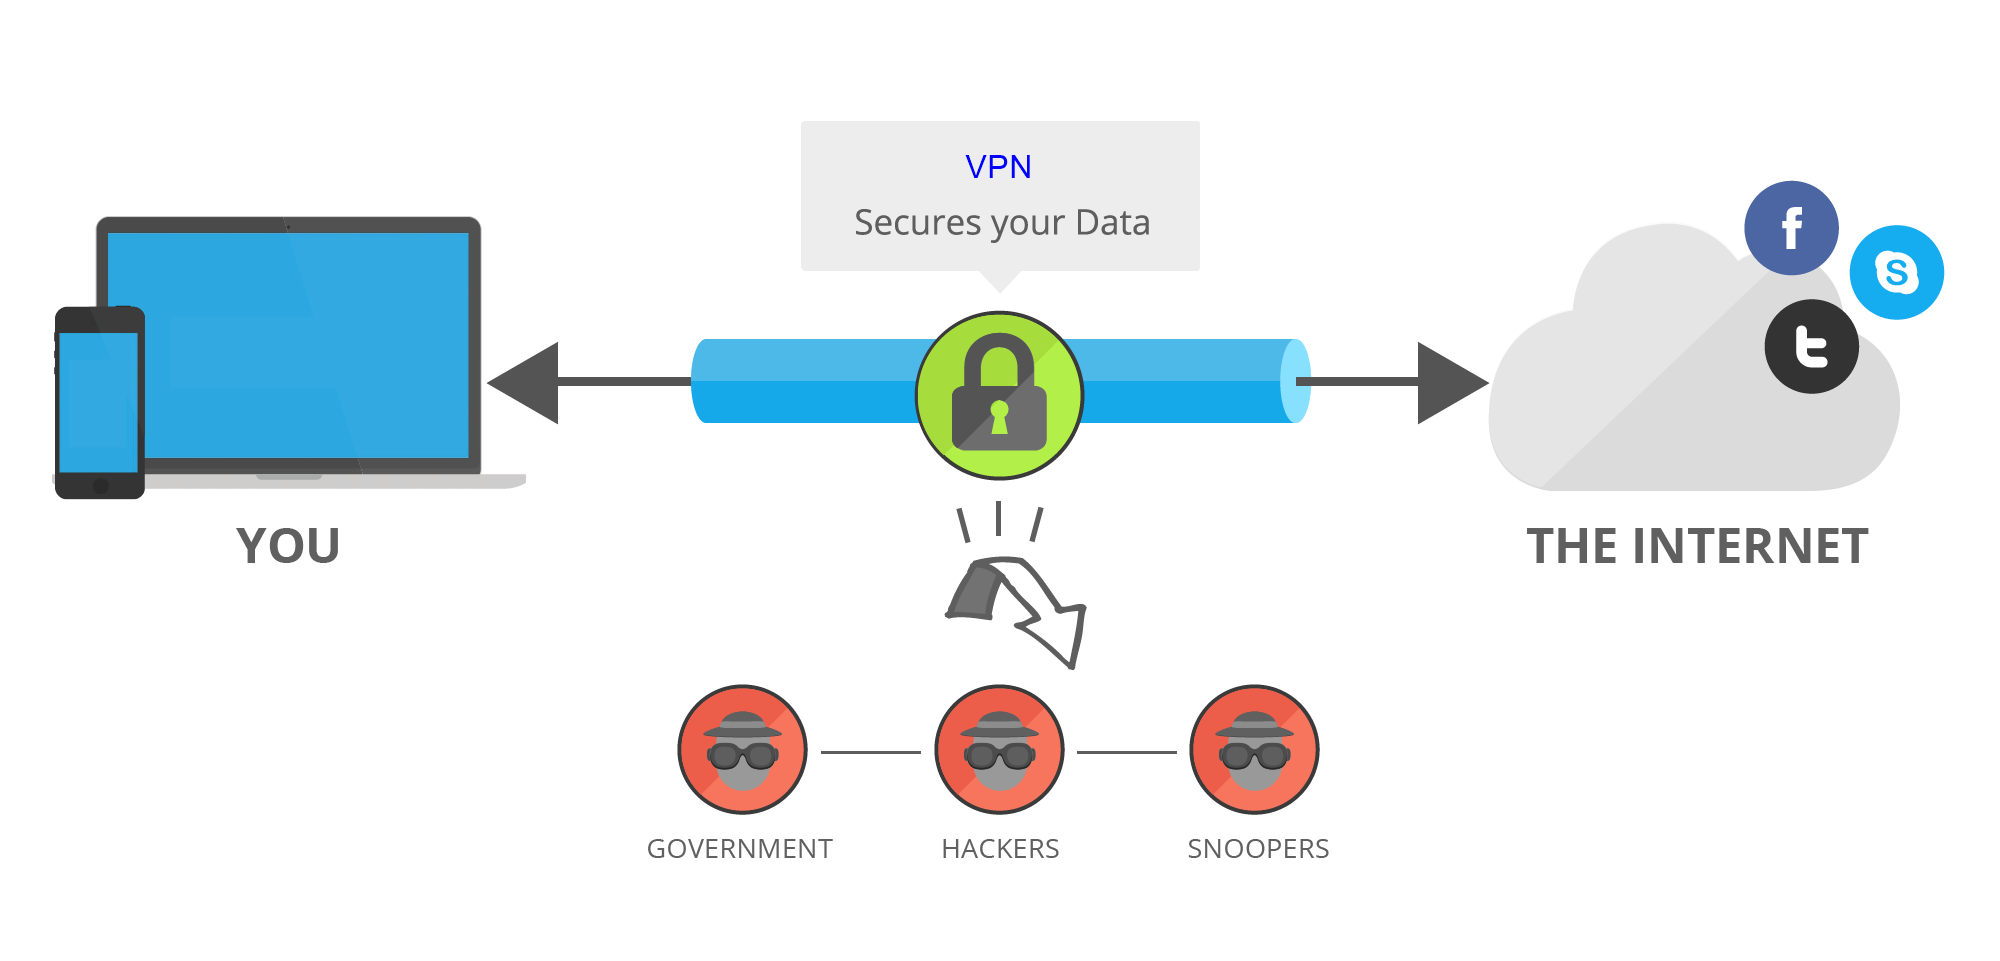
\includegraphics[width=0.7\textwidth]{img/VPN.png}
 		\caption{Funzionamento di una VPN \cite{68}.}
 	\end{figure}
 	
  	\afterpage{\blankpage}
  	
  	\chapter{Applicazioni}
  	\section{Costi e Implementazione}
 	Il numero di applicazioni real-time che utilizzano WebRTC al giorno d'oggi sono numerosissime, questo perché realizzarne una è molto semplice e non implica costi importanti. Fino a tredici anni fa, però, le cose erano completamente diverse; infatti la creazione di un servizio di comunicazioni richiedeva, oltre alla realizzazione delle infrastrutture server, lo sviluppo di applicazioni per ogni piattaforma o 
  	sistema operativo che avesse un numero di utenti non trascurabile. Ignorandone uno di questi comportava il rischio di non riuscire a raggiungere un livello di adozione sufficiente ad alimentare un business sostenibile. $\\$
  	La struttura di WebRTC e l'evoluzione dei browser hanno cambiato tutto questo; infatti la possibilità di effettuare connessione real-time peer-to-peer ha permesso a qualunque sviluppatore con capacità anche elementari di programmazione Web di realizzare un servizio di comunicazione real-time, audio e video. L’investimento richiesto sarà notevolmente più basso, in quanto basterà acquistare un semplice servizio in Web-hosting \cite{31}. $\\$
  	\begin{figure}[h!]
  		\centering
  		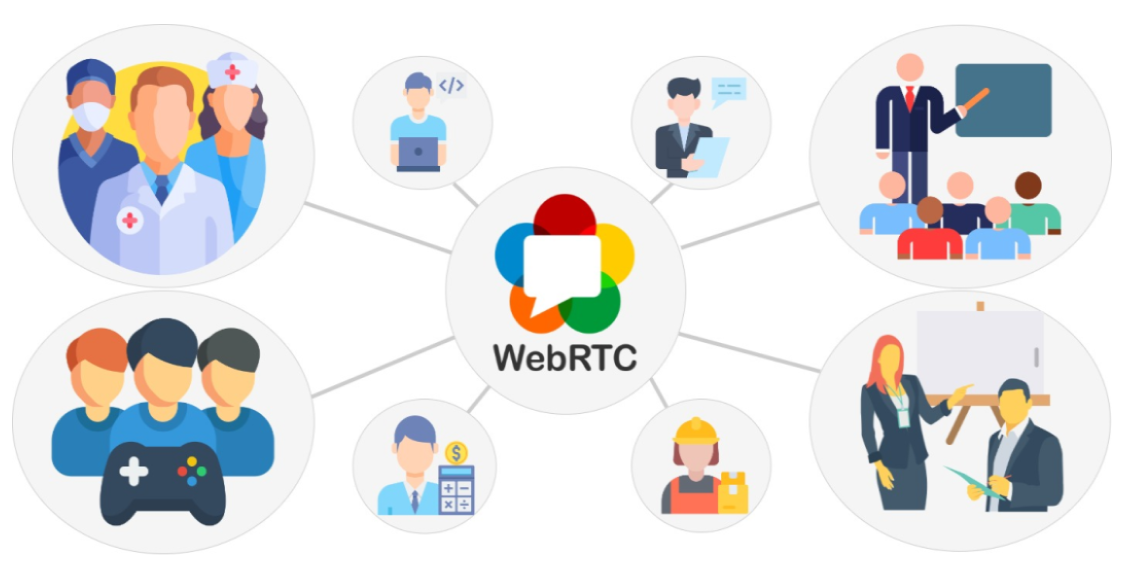
\includegraphics[width=0.7\textwidth]{img/applicazioni.png}
  		\caption{utilizzo di WebRTC nei principali ambiti \cite{69}.}
  	\end{figure}
  	
  	
  	\newpage
  	
  	\section{Casi d'Uso}
  	\subsection{Riunioni e Didattica a Distanza}
  	Dopo la sua creazione, WebRTC ha sempre più acquisito fama grazie al suo facile impiego per effettuare chiamate standard o videochiamate. Il suo utilizzo è impennato, però, all'inizio del 2020, con l'arrivo della pandemia del Covid-19; infatti questa tecnologia ha permesso a studenti e lavoratori di continuare le proprie attività nonostante l'isolamento in casa.$\\$
    Nel contesto scolastico WebRTC facilita la creazione di aule virtuali, offrendo lezioni coinvolgenti in tempo reale. Gli educatori possono utilizzare streaming video e audio, lavagne interattive e funzionalità di chat per condurre ambienti di apprendimento virtuale. Gli studenti possono partecipare attivamente, porre domande e collaborare con i compagni, favorendo un'esperienza educativa dinamica e interattiva. Inoltre è possibile effettuare sessioni individuali tra professore e studente; con gli strumenti appena citati, un insegnante può offrire una guida personalizzata ed esperienze di apprendimento interattive allo studente \cite{36}. 
  	\begin{figure}[h!]
  		\centering
  		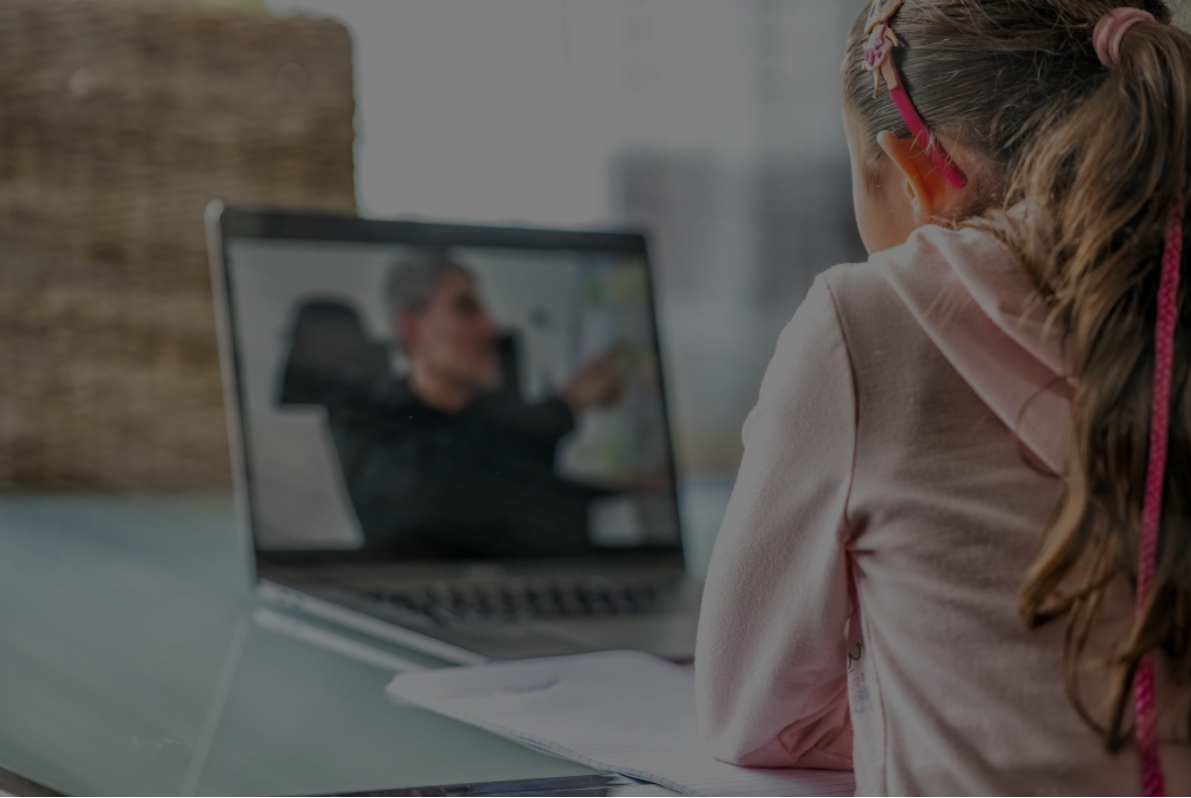
\includegraphics[width=0.5\textwidth]{img/didattica.png}
  		\caption{eLearning \cite{70}.}
  	\end{figure} 
  	Durante la pandemia, inoltre, un grande numero di aziende ha deciso di continuare ad operare optando per lo Smart Working, ovvero lavorare da casa senza doversi recare in ufficio. Anche in questo ambito WebRTC è una scelta più che azzeccata per effettuare chiamate/videochiamate che consentono ai dipendenti di lavorare tra loro o di svolgere riunioni. 
  	\begin{figure}[h!]
  		\centering
  		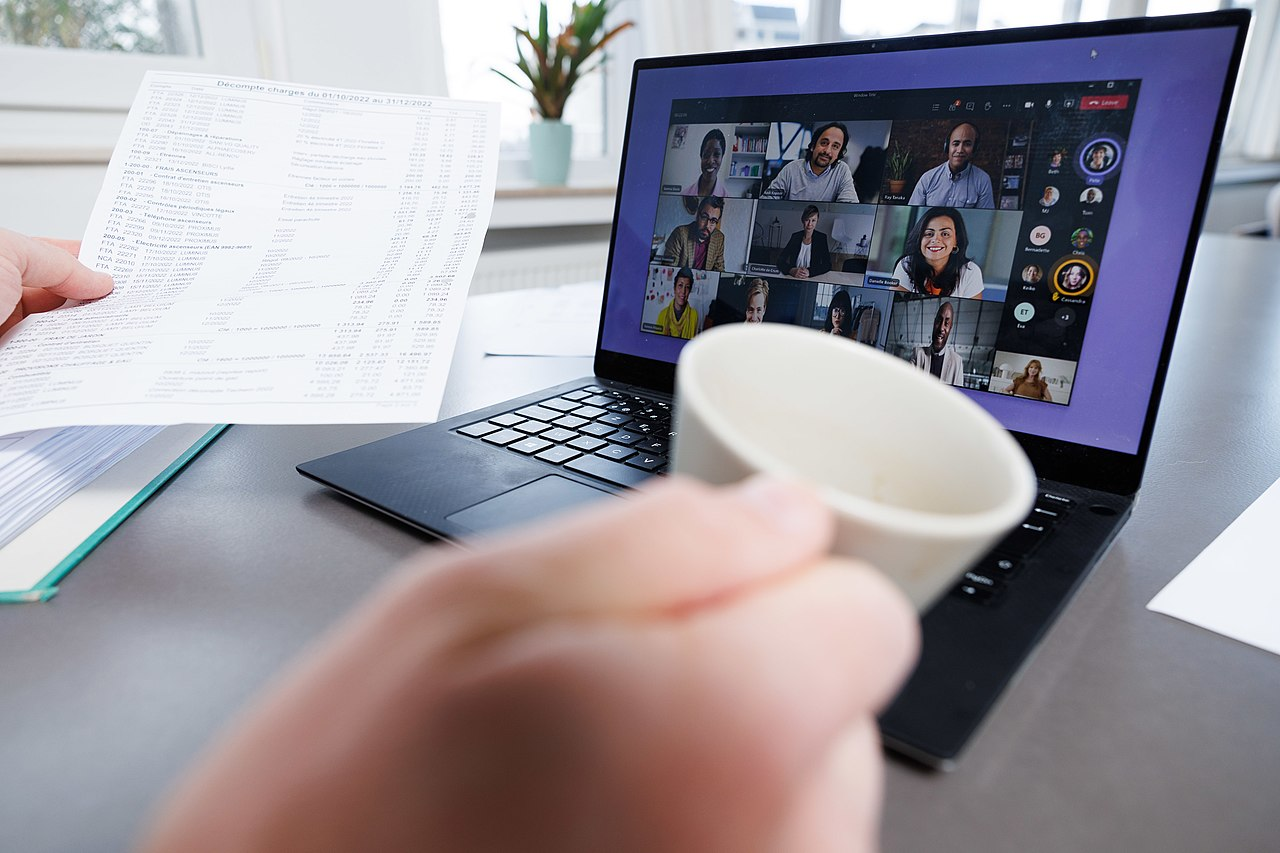
\includegraphics[width=0.5\textwidth]{img/smartworking.jpg}
  		\caption{Una riunione effettuata in remoto \cite{71}.}
  	\end{figure}
  	\newpage
  	
  	\subsection{IoT}
  	Quando si parla di Internet of Things si intendono tutti quegli oggetti fisici dotati di sensori, capacità di elaborazione, software e altre tecnologie che si connettono e scambiano dati con altri dispositivi e sistemi tramite Internet o altre reti di comunicazione. Il campo si è evoluto grazie alla convergenza di più tecnologie, tra cui sensori di merci, sistemi embedded sempre più potenti e machine learning \cite{37}.$\\$
  	Tra tutte queste tecnologie ha trovato impiego anche WebRTC, la cui applicazione in IoT è divisa in due gruppi: Device-to-Person e Device-to-Cloud. Nel primo gruppo rientrano tutte quelle applicazioni che consentono agli utenti di vedere o ascoltare cosa sta succedendo dall'altra parte come, per esempio, telecamere di sicurezza, video citofoni e babymonitor.$\\$ In Device-to-Cloud rientrano i casi di automazione. Ad esempio, la combinazione di WebRTC e IoT è adatta a qualsiasi ambito in cui, ad esempio, i droni identificano malfunzionamenti e forniscono un controllo completo, garantendo il flusso del processo in tempo reale \cite{38}.$\\$
  	Gli use cases di WebRTC nell'Internet of Things sono vari, ma i due casi principali sono quello per Smart Home e quello in ambito industriale. Nell'ambito delle Smart Home, WebRTC può essere utilizzato per dispositivi citofonici o cassette postali intelligenti che utilizzano questa tecnologia per la comunicazione audio/video con applicazioni Web e mobile. Nel primo caso, i residenti delle smart home sono in grado di comunicare con i visitatori, assicurandosi che nessun caso di urgenza passi inosservato. Le caselle di posta intelligenti abilitate con la tecnologia WebRTC, invece, permettono di sbloccare le proprie caselle di posta da ufficio o anche quando si è in vacanza. Un altro esempio di IoT nelle smart home è Alexa Echo. Tramite dispositivo si può utilizzare l'API RTCSessionController permettendo di comunicare con tutti gli altri dispositivi Echo presenti in casa (Immagine) [39]. $\\$
  	L'uso di WebRTC nel contesto industriale può essere molto utile per le operazioni di sorveglianza sui macchinari, rilevando tramite sensori possibili malfunzionamenti e avvisare gli operatori in tempo reale con WebRTC. Infatti l'applicazione più comune prevede il rilevamento di qualsiasi aumento insolito della temperatura delle macchine e ricercare le possibili cause come fumo dalla macchina, scintille che possono provocare incendi o sovraccarico. Con l'aiuto di WebRTC e sensori collegati alle macchine, gli avvisi possono essere inviati sotto forma di audio o video live, prevenendo così incidenti gravi. Inoltre, come già citato, il lavoro di rilevamento può essere migliorato tramite l'utilizzo di droni, che possono inviare riprese video in diretta che possono poi essere valutate e gestite di conseguenza (esempio) [39].
  	
  	\newpage
  	
  	\subsection{Assistenza sanitaria}
  	Nell'ambito sanitario l'utilizzo di WebRTC è vario. Il campo più importante in cui può intervenire WebRTC è la telemedicina. La telemedicina è l'insieme di tecniche mediche e informatiche che consentono la cura di un paziente a distanza o più in generale di fornire servizi sanitari a distanza, permettendo di superare le barriere geografiche ed aiutare le comunità rurali svantaggiate, per la mancanza di accesso all'assistenza sanitaria. In questo ambito WebRTC viene utilizzato per creare applicazioni di comunicazione real-time come \cite{38}:
  	\begin{itemize}
		\item Teleconferenza appuntamenti medico-paziente.
		\item Sedute di terapia a distanza.
		\item Teleconferenze di terapia di gruppo.
		\item Incontri clinici.
		\item Osservazione a distanza delle sale operatorie.
  	\end{itemize} 
  	La possibilità di utilizzare WebRTC in qualsiasi momento senza dover installare nessuna applicazione terza e la sicurezza crittografica che garantisce di salvaguardare i dati sanitari personali dei pazienti rappresentano per gli operatori sanitari dei punti a favore per l'utilizzo di WebRTC.
  	\begin{figure}[h!]
  		\centering
  		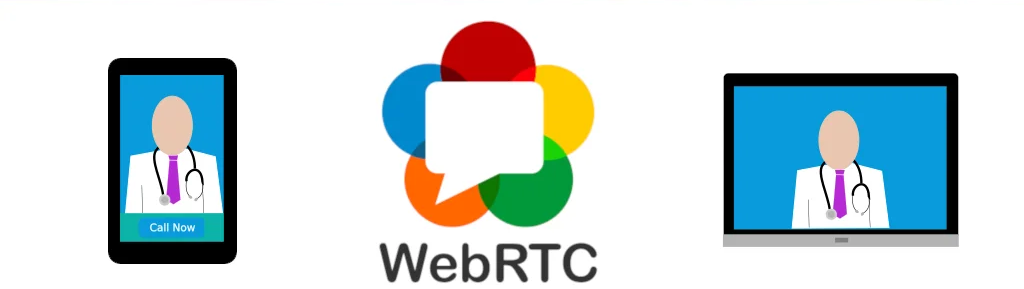
\includegraphics[width=0.7\textwidth]{img/telemedicina.jpg}
  		\caption{Telemedicina con WebRTC.}
  	\end{figure} $\\$
  	Un altro utilizzo è rivolto ai dispositivi indossabili come FitBit o Apple Watch; infatti questi salvano vite allertando, tramite WebRTC, il contatto di emergenza degli utenti e il pronto soccorso ogni volta che si verifica un picco o un calo improvviso della frequenza cardiaca \cite{39}.
  	
	\newpage
	
	
	\subsection{Giochi Multiplayer}
	Il mondo videoludico è uno dei più importanti contesti applicativi di WebRTC, che viene utilizzato principalmente per creare una comunicazione real-time nei giochi multiplayer su un browser. Prima dell'invenzione di WebRTC, la tecnologia maggiormente utilizzata per creare una connessione su un browser game era WebSocket che, grazie alla sua struttura, permetteva a due o più utenti di giocare assieme. WebSocket però utilizza TCP come protocollo di trasporto e, come abbiamo già visto, questo protocollo rende la comunicazione affidabile; nel contesto dei giochi multiplayer viene preferita una connessione UDP perché il fattore più importante non è l'arrivo assicurato e ordinato dei dati, bensì che questi siano spediti velocemente. Nonostante ciò, WebSocket gioca um ruolo importante per la fase di signaling tra gli utenti \cite{40}.$\\$
	Un altro importante utilizzo è quello riguardante il cloud gaming, un tipo di servizio online che esegue videogiochi su server remoti e li trasmette direttamente al dispositivo di un utente. I tre principali tipi di cloud gaming sono i giochi peer-to-peer, lo streaming dei giochi e il download progressivo \cite{41}. In questo ambiente WebRTC è un'ottima scelta applicativa per la sua bassa latenza e per il fatto di essere provato e testato in molte grandi applicazioni in tempo reale con miliardi di utenti, come Google Meets, Discord, Facebook Manager e altre. Il funzionamento è molto simile ad una videochiamata, con la differenza che un utente si collegherà tramite una connessione peer-to-peer ad un'istanza di gioco \cite{42}:
	\begin{figure}[h!]
		\centering
		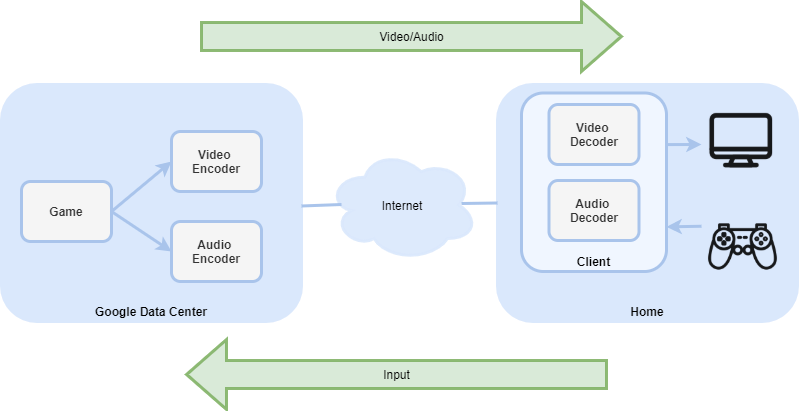
\includegraphics[width=0.7\textwidth]{img/Cloud.png}
		\caption{Architettura di Stadia, ex piattaforma di cloud gaming \cite{72}.}
	\end{figure} $\\$
	Nell'architettura di questa immagine si nota che quando un giocatore esegue un comando dal controller, questo viene spedito tramite i canali dati al servizio di cloud gaming, qui verrà elaborato e riprodotto. I segnali video ed audio vengono codificati e spediti tramite RTCPeerConnection; una volta arrivati sono decodificati dal dispositivo dell'utente \cite{42}.

	
	
	\newpage
	
  	\section{WebRTC contro tutti}
  	WebRTC non è l'unico strumento per creare applicazioni di comunicazioni real-time; infatti la concorrenza è grande e una delle tecnologie rivali più utilizzata è RTMP. Come abbiamo visto all'inizio, questo protocollo utilizzato sia da software (come OBS) che siti web (come YouTube) si basa su TCP. La scelta tra RTMP e WebRTC dipende dalle esigenze dello sviluppatore, considerando i punti di forza e limiti di entrambe le tecnologie: se da un lato WebRTC offre una migliore latenza, notevolmente più bassa rispetto a quella di RTMP, grazie all'utilizzo di UDP, dall'altro RTMP garantisce una maggiore scalabilità,  migliorando l'esperienza di visualizzazione agli utenti e consentendo ai server locali di memorizzare nella cache i contenuti in streaming \cite{43}. Entrambe le tecnologie hanno un alto livello di sicurezza: abbiamo già visto che WebRTC utilizza SRTP e DTLS per crittografare messaggi e per l'autenticazione. RTMP utilizza una sua variante, RTMPS, che permette di aggiungere un livello di sicurezza extra, che può essere TSL o SSL, per prevenire accessi non autorizzati. Infine è importate sottolineare che RTMP oltre al live streming viene utilizzato in pochissimi altri casi, a differenza di WebRTC che, come si è visto in precedenza, può essere implementato in più ambienti con successo \cite{43}.
  	\begin{figure}[h!]
  		\centering
  		
\includegraphics[width=0.9\textwidth]{img/RTCvsRTMP1.png}
  		\caption{WebRTC vs RTMP.}
  	\end{figure} $\\$ $\\$
  	Un'altra tecnologia di streaming audio e video concorrente di WebRTC è HLS, un protocollo di streaming a bitrate adattivo (una tecnica che funziona rilevando la larghezza di banda e la capacità della CPU di un utente in tempo reale, regolando di conseguenza la qualità del flusso multimediale) sviluppato da Apple, ampiamente utilizzato per lo streaming live su dispositivi mobili e browser desktop. HLS è progettato per funzionare con il protocollo HTTP e può essere facilmente integrato nell'infrastruttura basata su HTTP esistente. Le differenze tra HLS e WebRTC non sono molto diverse di quelle tra RTMP e WebRTC. Infatti HLS utilizza TCP come protocollo di trasporto, quindi ha una latenza più alta rispetto a WebRTC. A livello di sicurezza HLS utilizza HTTPS con TSL, garantendo un'autenticazione, protezione della privacy e integrità dei dati \cite{44}. Per quanto riguarda la compatibilità, HLS risulta una migliore scelta di WebRTC solamente su dispositivi e browser Apple, mentre nei restanti casi WebRTC è più funzionale \cite{45}.
  	
  	\newpage
  	\subsection{Teams vs Zoom}
  	Teams e Zoom sono tra le applicazioni più utilizzate al mondo che forniscono servizi gratuiti o a pagamento per effettuare chiamate e videochiamate con un grande numero di utenti. La prima è un'applicazione creata da Microsoft nel 2017; la seconda è stata rilasciata dall'azienda Zoom Video Communications nel 2011. Le differenze principali tra queste due è l'utilizzo di WebRTC da parte di Teams; infatti questa applicazione può essere utilizzata anche via browser, mentre per utilizzare Zoom è necessario installare la corrispettiva applicazione. altre differenze sono le seguenti \cite{46}:
  	\begin{itemize}
  		\item l'abbonamento gratuito di Teams supporta riunioni fino a 30 ore tra due persone oppure di 1 ora con un massimo di 100 utenti, un tempo migliore del piano gratuito di Zoom, che consente riunioni tra 100 utenti per un massimo di 40 minuti \cite{47}. Se si guardano tutti gli abbonamenti si nota come Teams sia una soluzione migliore per riunioni tra molte persone; infatti, a differenza di Zoom, permette di fare Webinar con 1000 utenti ed eventi in diretta con un massimo di 20000 partecipanti \cite{48}.
  		\item Un difetto di Teams è il cospicuo utilizzo di RAM, che può rallentare in modo sensibile una macchina con poca memoria. Zoom invece richiede un utilizzo di RAM inferiore quindi risulta una scelta migliore su computer poco potenti.
  		\item Su smartphone Zoom funziona in modo eccelso sia su Android che su iOS grazie all'aplicazione ben fatta e facile da utilizzare. Teams, invece, funziona senza problemi su Android, mentre il suo utilizzo su iOS non è possibile via Web; è necessario scaricare la relativa app \cite{49}.
  	\end{itemize} $\\$ $\\$
  	\begin{figure}[h!]
  		\centering
  		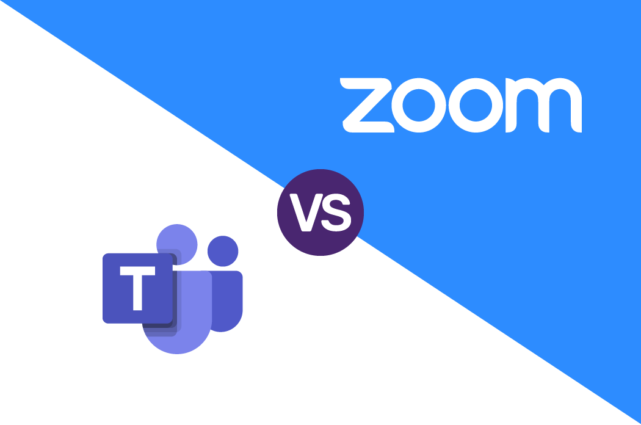
\includegraphics[width=0.5\textwidth]{img/TeamsvsZoom.png}
  		\caption{Teams vs Zoom \cite{73}.}
  	\end{figure}
  	\newpage
  	Altre differenze, come la dimensione dei file da trasferire, gestione dei documenti e altro vengono riportate nella seguente immagine: $\\$
  	\begin{figure}[h!]
  	 	\centering
  	 	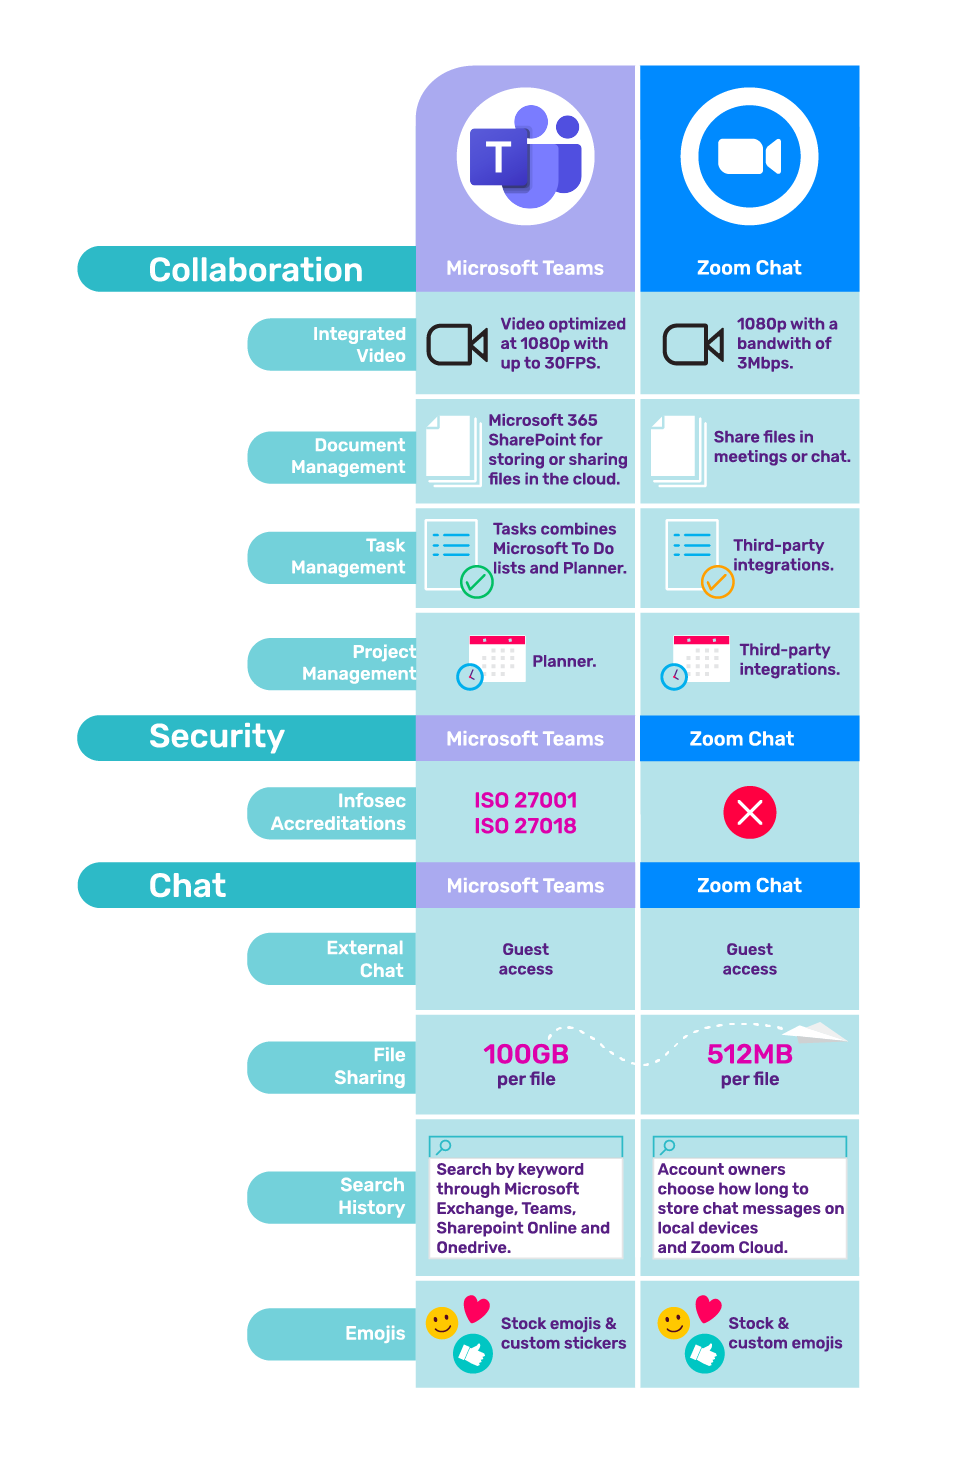
\includegraphics[width=0.6\textwidth]{img/Microsoft-Teams-vs-Zoom.png}
  	 	\caption{differenze tra Teams e Zoom \cite{73}.}
  	\end{figure} 
  	 
  	\afterpage{\blankpage}
  	 
  	\chapter{Progetto}
  	\section{Introduzione}
  	Il progetto proposto è una applicazione di videochiamata WebRTC tra due utenti con la possibilità di spedire file in totale sicurezza. E’ infatti garantita la privacy dei dati dal certificato SSL,
  	indispensabile per l’attivazione della connessione WebRTC. In conseguenza di tale propensione di WebRTC alla protezione dei dati personali, una sua possibile applicazione è nel campo della telemedicina nel trasferimento dei dati tra un dottore ed un paziente. In questo caso WebRTC consente di effettuare una videochiamata e di spedire file testuali con relative informazioni mediche del paziente (come, per esempio, la temperatura corporea, le pulsazioni, l’elettrocardiogramma, l’ossimetria e altro) per far si che un dottore possa verificare lo stato del suo paziente.$\\$
  	E' possibile visionare il funzionamento del progetto cliccando \textcolor{blue}{\href{https://www.youtube.com/watch?v=CIS8a7rEtUc}{qui}}.    
  	
  	\section{Strumenti utilizzati}
	Per la realizzazione dell'applicazione sono stati utilizzati i due linguaggi Javascript (per il funzionamento) e HTML (per la pagina web). Il codice è stato scritto su Visual Studio Code, un editor di codice sorgente sviluppato da Microsoft. Per la fase di signaling è stato utilizzato Firebase, una piattaforma per la creazione di applicazioni per dispositivi mobili e web sviluppata da Google [https://it.wikipedia.org/wiki/Firebase]. Grazie a questa piattaforma è possibile creare un progetto con un database Firestore (un database flessibile e scalabile per lo sviluppo di dispositivi mobili, Web e server da Firebase) e collegarlo alla propria applicazione JS. Firebase è stato preferito a WebSocket perché a livello di codice è più semplice e veloce da implementare; inoltre ha funzioni di notifica utente ogni volta che avviene un cambiamento all'interno del DB Firestore.
	
	\newpage
	 
  	\section{Funzionamento}
  	\subsection{Creazione Certificato SSL}
  	Prima di analizzare il funzionamento del progetto è necessario parlare dei certificati SSL. Il motivo per il quale un certificato diventa indispensabile in un'applicazione WebRTC è l'API getUserMedia perché, con l'uscita di Chrome 47 (2015), quest'API non è più supportata su pagine HTTP, ma solo su pagine HTTPS; infatti se utilizzata su pagina HTTP, getUserMedia restituirà un errore (NotAllowedError), cosa che non accade su una pagina HTTPS \cite{77}. getUserMedia però verifica solamente che la pagina sia HTTPS, senza controllare se il certificato sia approvato da una Certification Authority; quindi basta generare un certificato affinché l'applicazione funzioni. $\\$
  	Per la creazione del certificato sono state utilizzate tre funzioni di OpenSSL (uno strumento da riga di comando open source che consente agli utenti di eseguire varie attività relative a SSL) \cite{78}:
  	\begin{itemize}
  		\item La prima serve per generare una chiave privata RSA a 256 Byte utilizzata per abilitare la crittografia, salvando nel file domain.key.
  		\begin{lstlisting}
    	openssl genrsa -out domain.key 2048
  		\end{lstlisting}
  		\item Una volta creata la chiave privata è necessario creare una Certificate Signing Request (CSR) ovvero una comunicazione inviata ad una Certificate Authority al fine di ottenere un certificato di identità digitale \cite{79}. La funzione di OpenSSL utilizzata è la seguente
  		\begin{lstlisting}
  	openssl req -key domain.key -new -out domain.csr
  		\end{lstlisting}
  		\item L'ultima funzione è quella per creare un certificato autofirmato con la chiave privata e la CSR. Può essere utilizzato per crittografare i dati così come i certificati firmati dalla CA, ma agli utenti verrà mostrato un avviso che informa che il certificato non è attendibile. 
  		\begin{lstlisting}
	openssl x509 -signkey domain.key -in domain.csr -req -days 365 
						       -out domain.crt
  		\end{lstlisting}
  	\end{itemize}
  	\newpage
  	
  	
  	\subsection{Lato Server}
  	Una volta creato il certificato SSL è possibile implementarlo nella pagina attraverso il file index.js che gestisce il lato server. Le principali funzioni utilizzate sono express, fs (file system) e https. Express, un framework per applicazioni web per Node.js, progettato per creare web application e API, viene utilizzato per due motivi: con il metodo get dice al server cosa fare quando viene chiamata una richiesta get sulla route specificata [https://expressjs.com/it/guide/routing.html]; i metodi use e static permettono di fornire al server i file nella cartella public (in questo caso style.css, client.js e main.js) [https://expressjs.com/en/starter/static-files.html]. Il framework fs ci permette di effettuare operazioni sui file presenti nel computer, come Leggere, Creare, Aggiornare, Cancellare e Rinominare i file. Il metodo readFileSync viene utilizzato per leggere il contenuto della chiave e del certificato per restituirlo nelle apposite variabili [https://www.geeksforgeeks.org/node-js-fs-readfilesync-method/]. Infine https viene utilizzata per creare il server con chiave, certificato e funzione di callback, mettendolo in ascolto sulla porta specificata (in questo caso la 8081). 
  	\begin{lstlisting}
  		var express = require('express');
  		var app = express();
  		var https = require('https')
  		const fs = require('fs')
  		
  		app.get('/', function (req, res) {
  			fs.createReadStream('index.html').pipe(res)
  		})
  		
  		app.use(express.static('public'))
  		
  		var privKey = fs.readFileSync('certificates/domain.key')
  		var cert = fs.readFileSync('certificates/domain.crt')
  		
  		
  		https.createServer({
  			key: privKey,
  			cert: cert,
  			passphrase: 'qwerty'
  		}, app).listen(8081);
  	\end{lstlisting}$\\$
  
  	\newpage
  	
  	\subsection{Lato Client}
  	Client.js è il file che fornisce il funzionamento dell'applicativo. Questo è suddiviso in due parti: la prima riguarda la dichiarazione e creazioni di variabili; le prime riguardano il collegamento del nostro progetto a Firebase, inserendo nella variabile firebaseConfig le informazioni che si trovano nella applicazione web creata sul sito di Firebase e richiamando il metodo initializeApp, e al database Firestore. Successivamente ci sono le variabili per la connessione peer (servers contiene i server STUN che verranno utilizzati durante la fase ICE) e quelle per accedere agli stream audio e video degli utenti; infine vengono dichiarate le variabili per gestire gli elementi HTML. $\\$
  	\begin{lstlisting}[
  		basicstyle=\small  		]
  		const firebaseConfig = {
  			apiKey: "GbRTScPBmV5IWaTt-kqxCV561bWJ4z7TRIlKpEu0Mo",
  			authDomain: "videocall-150f7.firebaseapp.com",
  			databaseURL: "https://videocall-150f7-default-rtdb.
  								firebaseio.com",
  			projectId: "videocall-150f7",
  			storageBucket: "videocall-150f7.appspot.com",
  			messagingSenderId: "543562675407",
  			appId: "1:157235812407:web:6OP11aa5ab27vPaLae8b708"
  		};
  		
  		firebase.initializeApp(firebaseConfig)
  		
  		const firestore = firebase.firestore();
  		
  		const servers = {
  			iceServers: [
  			{
  				urls: ['stun:stun1.l.google.com:19302', 
  					   'stun:stun2.l.google.com:19302'],
  			},
  			],
  			iceCandidatePoolSize: 10,
  		};
  		
  		let pc;
  		let localStream = null;
  		let remoteStream = null;
  		
  		//HTML variables
  		...
  	\end{lstlisting}$\\$
  	La seconda parte riguarda il funzionamento dei vari pulsanti. Il primo gestisce l'accesso ai dispositivi dell'utente; prima di tutto viene creata la connessione peer tramite RTCPeerConnection, necessario per aggiungere le tracce audio e video alla variabile pc. Seguono poi le operazioni sugli stream locale e remoto. Sul primo richiamiamo il metodo getUserMedia per chiedere all'utente di concedere l'autorizzazione ad accedere al suo microfono e webcam; se concessa, tutte le tracce ottenute su localStream vengono aggiunte sulla variabile pc.
  	Lo stream remoto invece viene creato e riempito con tracce vuote tramite l'EventHandler ontrack di RTCPeerConnection (ogni volta che una traccia viene aggiunta alla variabile pc, ontrack viene lanciato eseguendo la funzione specificata). infine aggiungiamo i due stream alle variabili che gestiscono gli elementi video HTML.
  		\begin{lstlisting}[
  		basicstyle=\small  		]
  		webcamButton.onclick = async () => {
  			pc = new RTCPeerConnection(servers);
  			
  			localStream = await navigator.mediaDevices.getUserMedia({ 
  				video: true, audio: true }) 
  			remoteStream = new MediaStream()
  	
  			localStream.getTracks().forEach((track) => {
  				pc.addTrack(track, localStream)
  			}); 
  			
  			pc.ontrack = (event) => {
  				event.streams[0].getTracks().forEach((track) => {
  					remoteStream.addTrack(track)
  				});
  			};
  			
  			webcamVideo.srcObject = localStream;
  			remoteVideo.srcObject = remoteStream;
  		};
  	\end{lstlisting}$\\$
  	Una volta date le autorizzazione per accedere ai propri dispositivi, l'utente può creare una chiamata oppure partecipare ad una già esistente. Nel primo caso deve premere il pulsante "Crea chiamata"; il processo per creare un'offerta è il seguente: una volta premuto il bottone, vengono istanziate tre variabili per collegarsi alle collezioni del database Firestore che riguardano le chiamate e i candidati ICE dei due utenti (il database è strutturato in modo che per ogni chiamata corrisponda un identificativo al quale sono associati offerta, risposta e candidati ICE). Successivamente viene generato un id casuale tramite la proprietà .id di firestore: questo verrà utilizzato come id della chiamata. La prossima istruzione serve per ottenere e scrivere sul database i candidati ICE del chiamante. Una volta fatto ciò viene creata l'offerta tramite il metodo createOffer (di RTCPeerConnection) e impostata come descrizione locale; le sue informazioni vengono inserite nella variabile offer che successivamente verrà scritta sul database. Infine sono presenti due listener onSnapshot: il primo fa si che se un utente risponde alla chiamata, la sua risposta venga impostata come descrizione remota se quest'ultima è vuota; il secondo invece aggiunge un nuovo candidato ICE del utente chiamato ogni volta che ne viene aggiunto uno sul database. $\\$
  	
  	\begin{lstlisting}[
  		basicstyle=\small]
  		callButton.onclick = async () => {
  			const callDoc = firestore.collection('calls').doc(); 
  			
  			const offerCandidates = callDoc.
  				collection('offerCandidates');
  			const answerCandidates = callDoc.
  				collection('answerCandidates');
  			
  			callInput.value = callDoc.id; 
  			
  			pc.onicecandidate = (event) => {
  				event.candidate && offerCandidates.add(event.
  							   candidate.toJSON());
  			};
  			
  			const offerDescription = await pc.createOffer();
  			await pc.setLocalDescription(offerDescription);  
  			
  			const offer = {
  				sdp: offerDescription.sdp,
  				type: offerDescription.type,
  			};
  			
  			await callDoc.set({ offer });
  		}
  	\end{lstlisting}$\\$
  	Il codice del pulsante per unirsi ad una chiamata è per la maggior parte identico al pulsante per creare una chiamata, con l'unica differenza che non si gestisce l'offerta, ma la risposta RTCPeerConnection. Dopo aver creato le variabili per il database e aggiunto i candidati ICE alla collezione answerCandidates, si prende dal database l'offerta e la si imposta come descrizione remota; successivamente si crea la risposta, la si imposta come descrizione locale e viene aggiunta al database. Anche qui è presente un listener per far si che ogni ICE del chiamante aggiunto al database venga aggiunto anche alla variabile RTCPeerConnection.  
  	
  	\begin{lstlisting}[basicstyle=\small]
  		answerButton.onclick = async () => {
  			const callId = callInput.value;
  			const callDoc = firestore.collection('calls').
  				doc(callId);
  			const answerCandidates = callDoc.
  				collection('answerCandidates');
  			const offerCandidates = callDoc.
  				collection('offerCandidates');
  			
  			pc.onicecandidate = (event) => {
  				event.candidate && answerCandidates.add(event.
  					candidate.toJSON());
  			};
  			
  			const callData = (await callDoc.get()).data();
  			const offerDescription = callData.offer;
  			await pc.setRemoteDescription(new 
  				RTCSessionDescription(offerDescription));
  			
  			const answerDescription = await pc.createAnswer();
  			await pc.setLocalDescription(answerDescription);
  			
  			const answer = {
  				type: answerDescription.type,
  				sdp: answerDescription.sdp,
  			};
  			
  			await callDoc.update({ answer });
  			
  			offerCandidates.onSnapshot((snapshot) => {
  				snapshot.docChanges().forEach((change) => {
  					console.log(change);
  					if (change.type === 'added') {
  						let data = change.doc.data();
  						pc.addIceCandidate(new 
  							RTCIceCandidate(data));
  					}
  				});
  			});
  		};
  	\end{lstlisting}
  	\newpage
  	Il quarto pulsante consente agli utenti di spedire i file con i dati diagnostici del paziente. Questo trasferimento è possibile grazie ad un Data Channel, impostato dal metodo createDataChannel di RTCPeerConnection. Una volta creato si gestisce l'evento onmessage, ovvero cosa deve fare il canale dati quando un messaggio viene spedito. Nel codice seguente osserviamo in particolare la funzione onMessageCallback nella quale, una volta che il file è stato spedito, viene creato nel browser di destinazione un nuovo Blob nel quale si caricano tutte le informazione del file ricevuto e successivamente si crea un link che, se cliccato, permette all'utente di scaricare il Blob appena creato.
  	\begin{lstlisting}[basicstyle=\small]
  		reciveBuffer = []
  		pc = new RTCPeerConnection(servers);
  		dataChannel = pc.createDataChannel('fileChannel', 
  				{ negotiated: true, id: 0 });
  		dataChannel.onmessage = onMessageCallback;
  		
  		function onMessageCallback(event) {
  			receiveBuffer.push(event.data);
  			
  			const receivedFile = new Blob(receiveBuffer);
  			receiveBuffer = [];
  			
  			downloadAnchor.href = URL.createObjectURL(receivedFile);
  			downloadAnchor.download = "temperatura.txt"
  			downloadAnchor.textContent =
  			`Click to download the file`;
  			downloadAnchor.style.display = 'block'; 
  			console.log("file ricevuto");
  		}
  	\end{lstlisting} $\\$
  	Nel pulsante di spedizione viene selezionato il file dall'elemento input HTML e tramite una variabile FileReader il contenuto del file viene letto, salvato su una variabile (data) e spedito tramite il metodo send di RTCDataChannel.
  	\begin{lstlisting}[basicstyle=\small]
  		sendButton.onclick = async () => {
  			const file = fileInput.files[0];
  			const reader = new FileReader();
  			
  			reader.onload = (event) => {
  				const data = event.target.result;
  				dataChannel.send(data);
  				console.log("file spedito");
  			};
  			
  			reader.readAsArrayBuffer(file);
  		}
  	\end{lstlisting}
  	\newpage
  	Infine, l'ultimo pulsante permette all'utente di riagganciare. Al suo interno viene semplicemente chiusa la connessione peer e il canale dati tramite il metodo close(), rimuove tutte le tracce dallo stream remoto e locale e si cancella l'ID della chiamata. $\\$
  	\begin{lstlisting}
  		hangupButton.onclick = async () => {
  			pc.close();
  			dataChannel.close();
  			
  			remoteStream.getTracks().forEach(function(track){
  				track.stop();
  			});
  			remoteVideo.srcObject = remoteStream;
  			
  			localStream.getTracks().forEach(function(track) {
  				track.stop();
  			});
  			webcamVideo.srcObject = localStream;
  			
  			callInput.value = "";
  		}
  	\end{lstlisting} $\\$

	\subsection{Webpack}
	Per includere il file client.js ho utilizzato Webpack, un module bundler, ovvero uno strumento per organizzare e combinare molti file in un unico file; viene solitamente utilizzato quando un progetto diventa troppo grande o quando lavoriamo con librerie che hanno più dipendenze e generano errori. Ed era proprio questo il problema del file client che webpack risolve creando un grafico delle dipendenze mentre analizza i file JS, tenendo traccia sia delle dipendenze dei file di origine che delle dipendenze di terze parti. Questo grafico garantisce che tutti i file di codice sorgente e associati siano aggiornati e privi di errori [https://www.gianlucatramontana.it/2023/04/04/i-module-bundler-in-javascript/]. per utilizzare Webpack si utilizza il comando sottostante; questo creerà un nuovo file (main.js) che, una volta inserito nel tag script di html, farà funzionare correttamente il programma senza alcun tipo di errore. Ovviamente questo operazione è da effettuare ogni volta che si fa una modifica sul file client.js.$\\$
	\begin{lstlisting}
			webpack ./public/client.js
	\end{lstlisting}

  	
  	\afterpage{\blankpage}
  	
 	\chapter{Conclusioni}
 	Questo documento ha analizzato la tecnologia WebRTC, dimostrando che cos'è, come funziona e quali sono le sue applicazioni. Infatti come abbiamo visto questa tecnologia nata 10 anni fa ha risolto un problema alla quale da tempo si cercava una soluzione: creare applicazioni di comunicazione in tempo reale utilizzandole via browser, quindi senza installare plugin o software terzi.$\\$
 	Il suo funzionamento si basa sull'utilizzo di pagine HTML, ma soprattutto di API Javascript, che permettono di utilizzare i dispositivi input audio e video dell'utente (MediaStream), creare una connessione con uno o più peer (RTCPeerConnection) e scambiare messaggi (RTCDataChannel). Utilizzando il protocollo UDP per il trasporto e la tecnologia ICE per trovare il percorso tra i due utenti, WebRTC consente una connessione veloce. La sicurezza è garantita grazie ai protocolli SRTP e DTLS, che crittano ed evitano l'intercettazione dei messaggi. Questo comunque non rende WebRTC completamente sicuro; infatti possono verificarsi delle perdite riguardanti gli IP degli utenti; l'utilizzo di una VPN, però, riduce sensibilmente questa potenziale falla nel sistema di sicurezza.$\\$
 	Dopo la sua creazione, tutti i browser e sistemi mobile si sono impegnati per renderlo utilizzabile tra browser differenti; infatti nel 2013 avviene la prima chiamata cross-browser. E' vero anche che i dispositivi Apple hanno iniziato a supportare questa tecnologia nel 2017 e ancora oggi risulta più problematica rispetto a quella su Android (per quanto riguarda iPhone) o su Chrome/FireFox (per quanto riguarda Safari).$\\$
 	Negli anni WebRTC ha trovato impiego in molti campi, primo fra tutti la didattica/lavoro a distanza.
 	Ci sono due campi in particolare dove WebRTC viene già utilizzato, ma ha ancora molte potenzialità per il futuro; si parla dell'IoT e della telemedicina. Oggi, grazie a questa tecnologia, è possibile effettuare operazioni di automazione industriale e di monitoraggio remoto tramite dispositivi IoT oppure sedute mediche a distanza tra paziente e dottore con la telemedicina. In questo ambiente WebRTC potrebbe un giorno essere utilizzato non solo per effettuare chiamate di controllo, ma anche per eseguire operazioni mediche di tipo chirurgico oppure di trapianto d'organi effettuate tramite, per esempio, l'accesso remoto a macchinari appositi. $\\$
 	Il progetto sviluppato in questa tesi ha mostrato le potenzialità di questo strumento di comunicazione in un ambiente controllato come quello tra medico e paziente. Come sviluppo futuro si potrebbe pensare di automatizzare il riconoscimento dei dispositivi di diagnostica collegati al paziente e fare in modo che in chiamata il medico possa vedere il paziente e contemporaneamente in una finestra laterale leggere i dati istantanei delle misure restituite dai vari dispositivi, quali termometro, pulsossimetro, elettrocardiografo ed altre informazioni.
 	
 	\afterpage{\blankpage}
 	
 	\appendix
 	\chapter{VP8}
 	Il VP8 (Video Compression Format o Video Compression Specification) è una specifica per la codifica e la decodifica di video ad alta definizione come file o bitstream per la visualizzazione rilasciata nel 2008. A differenza del suo omologo codec H.264, il codec VP8 è gratuito. Ciò è dovuto al fatto che Google ha rilasciato tutti i brevetti che possiede sotto una licenza pubblica royalty-free (un tipo di licenza che permette l'utilizzo di una risorsa con limitate restrizioni sul suo utilizzo e pagando una cifra iniziale estremamente contenuta.). H.264, tuttavia, contiene una tecnologia brevettata e richiede licenze da parte dei detentori di brevetti e royalty limitate per l’hardware. Opera, Firefox, Chrome e Chromium supportano la riproduzione di video VP8 nel tag video HTML5. Secondo Google, VP8 è utilizzato principalmente in connessione con WebRTC e come formato per brevi animazioni in loop, in sostituzione del Formato di interscambio grafico \cite{50}.
 	\begin{figure}[h!]
 		\centering
 		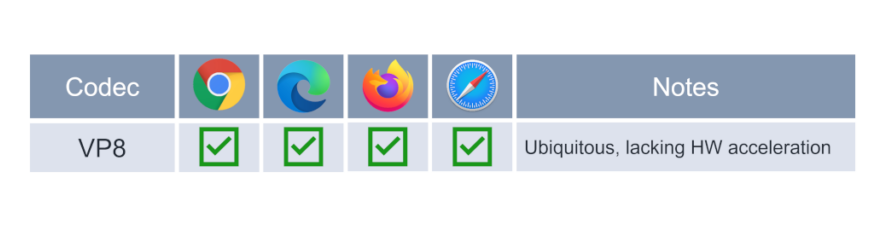
\includegraphics[width=0.7\textwidth]{img/VP8.png}
 		\caption{Supporto di VP8 sui browser principali \cite{74}.}
 	\end{figure}
 	\chapter{NAT}
 	Con NAT (Network Address Translation) si intendono tutti quei processi di modifica di uno o più indirizzi IP privati locali in un indirizzo IP pubblico globale tramite apparati di rete come router o firewall. Questo offre la possibilità di accedere a Internet con maggiore sicurezza e privacy nascondendo l'indirizzo IP del dispositivo dalla rete pubblica, anche durante l'invio e la ricezione di traffico. \cite{51}. Lo scopo principale del NAT è quello di ovviare alla scarsità di indirizzi IP pubblici disponibili; le tecniche utilizzate per effettuare queste operazioni rendono i dispositivi non direttamente raggiungibili da Internet, garantendo la sicurezza e privacy citata prima. Esistono sostanzialmente due tipi di NAT: il source NAT e il destination NAT; l'unica differenza tra questi due è la modifica dell'indirizzo del pacchetto che inizia una nuova connessione: nel primo caso viene modificato quello di sorgente, nel secondo quello di destinazione. Il tipo di NAT più utilizzato è PAT(Port Address Translation), un tipo di source NAT in cui gli indirizzi dei dispositivi di una rete privata vengono rappresentati verso l'esterno come un solo indirizzo IP. In questo tipo di NAT vengono modificate anche le porte TCP e UDP delle connessioni in transito (per questo il nome Port Address Translation) \cite{52}.
 	\begin{figure}[h!]
 		\centering
 		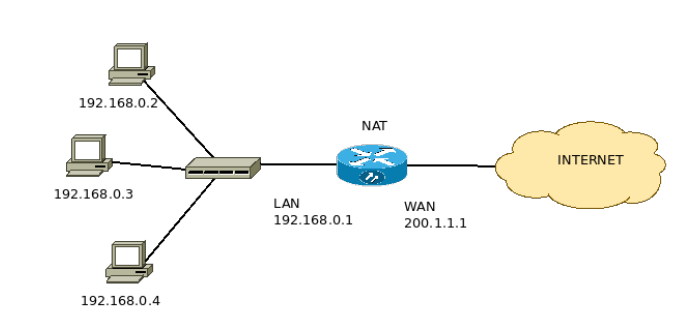
\includegraphics[width=0.7\textwidth]{img/nat.png}
 		\caption{Funzionamento del NAT \cite{75}.}
 	\end{figure}
 
 	\chapter{TLS}
 	Transport Layer Security (TLS) è un protocollo crittografico progettato per fornire la sicurezza delle comunicazioni su una rete di computer. Il protocollo è ampiamente utilizzato in applicazioni come e-mail, messaggistica istantanea e voice over IP. Il protocollo TLS mira principalmente a fornire sicurezza, l'integrità e l'autenticità attraverso l'uso della crittografia, come l'uso di certificati, tra due o più applicazioni informatiche comunicanti.Il Datagram Transport Layer Security (DTLS) strettamente correlato è un protocollo di comunicazione che fornisce sicurezza alle applicazioni basate su datagrammi \cite{53}.$\\$
 	TLS può funzionare sia con crittografia simmetrica che asimmetrica. Nel primo caso i messaggi vengono crittati con una chiave che conoscono solamente il mittente e il destinatario lunga 128 o 256 bit. Questo tipo di crittografia è efficiente a livello computazionale, ma lo scambio della chiave comune deve essere fatto in modo sicuro. Nella crittografia asimmetrica, mittente e destinatario hanno entrambi una coppia di chiavi: una pubblica ed una privata. Le chiavi pubbliche dei destinatari vengono utilizzate per crittografare i messaggi dai mittenti, mentre le chiavi private vengono utilizzate per decodificare. Con TLS asimmetrico non è presente lo scambio di chiavi tra i due utenti. Inoltre la chiave private è matematicamente correlata alla chiave pubblica, ma utilizzando chiavi sufficientemente lunghe sarà molto difficile dedurre la chiave privata da quella pubblica. Per questi motivi TLS asimmetrico è più sicuro di TLS simmetrico e anche più utilizzato \cite{54}.
 	\begin{figure}[h!]
 		\centering
 		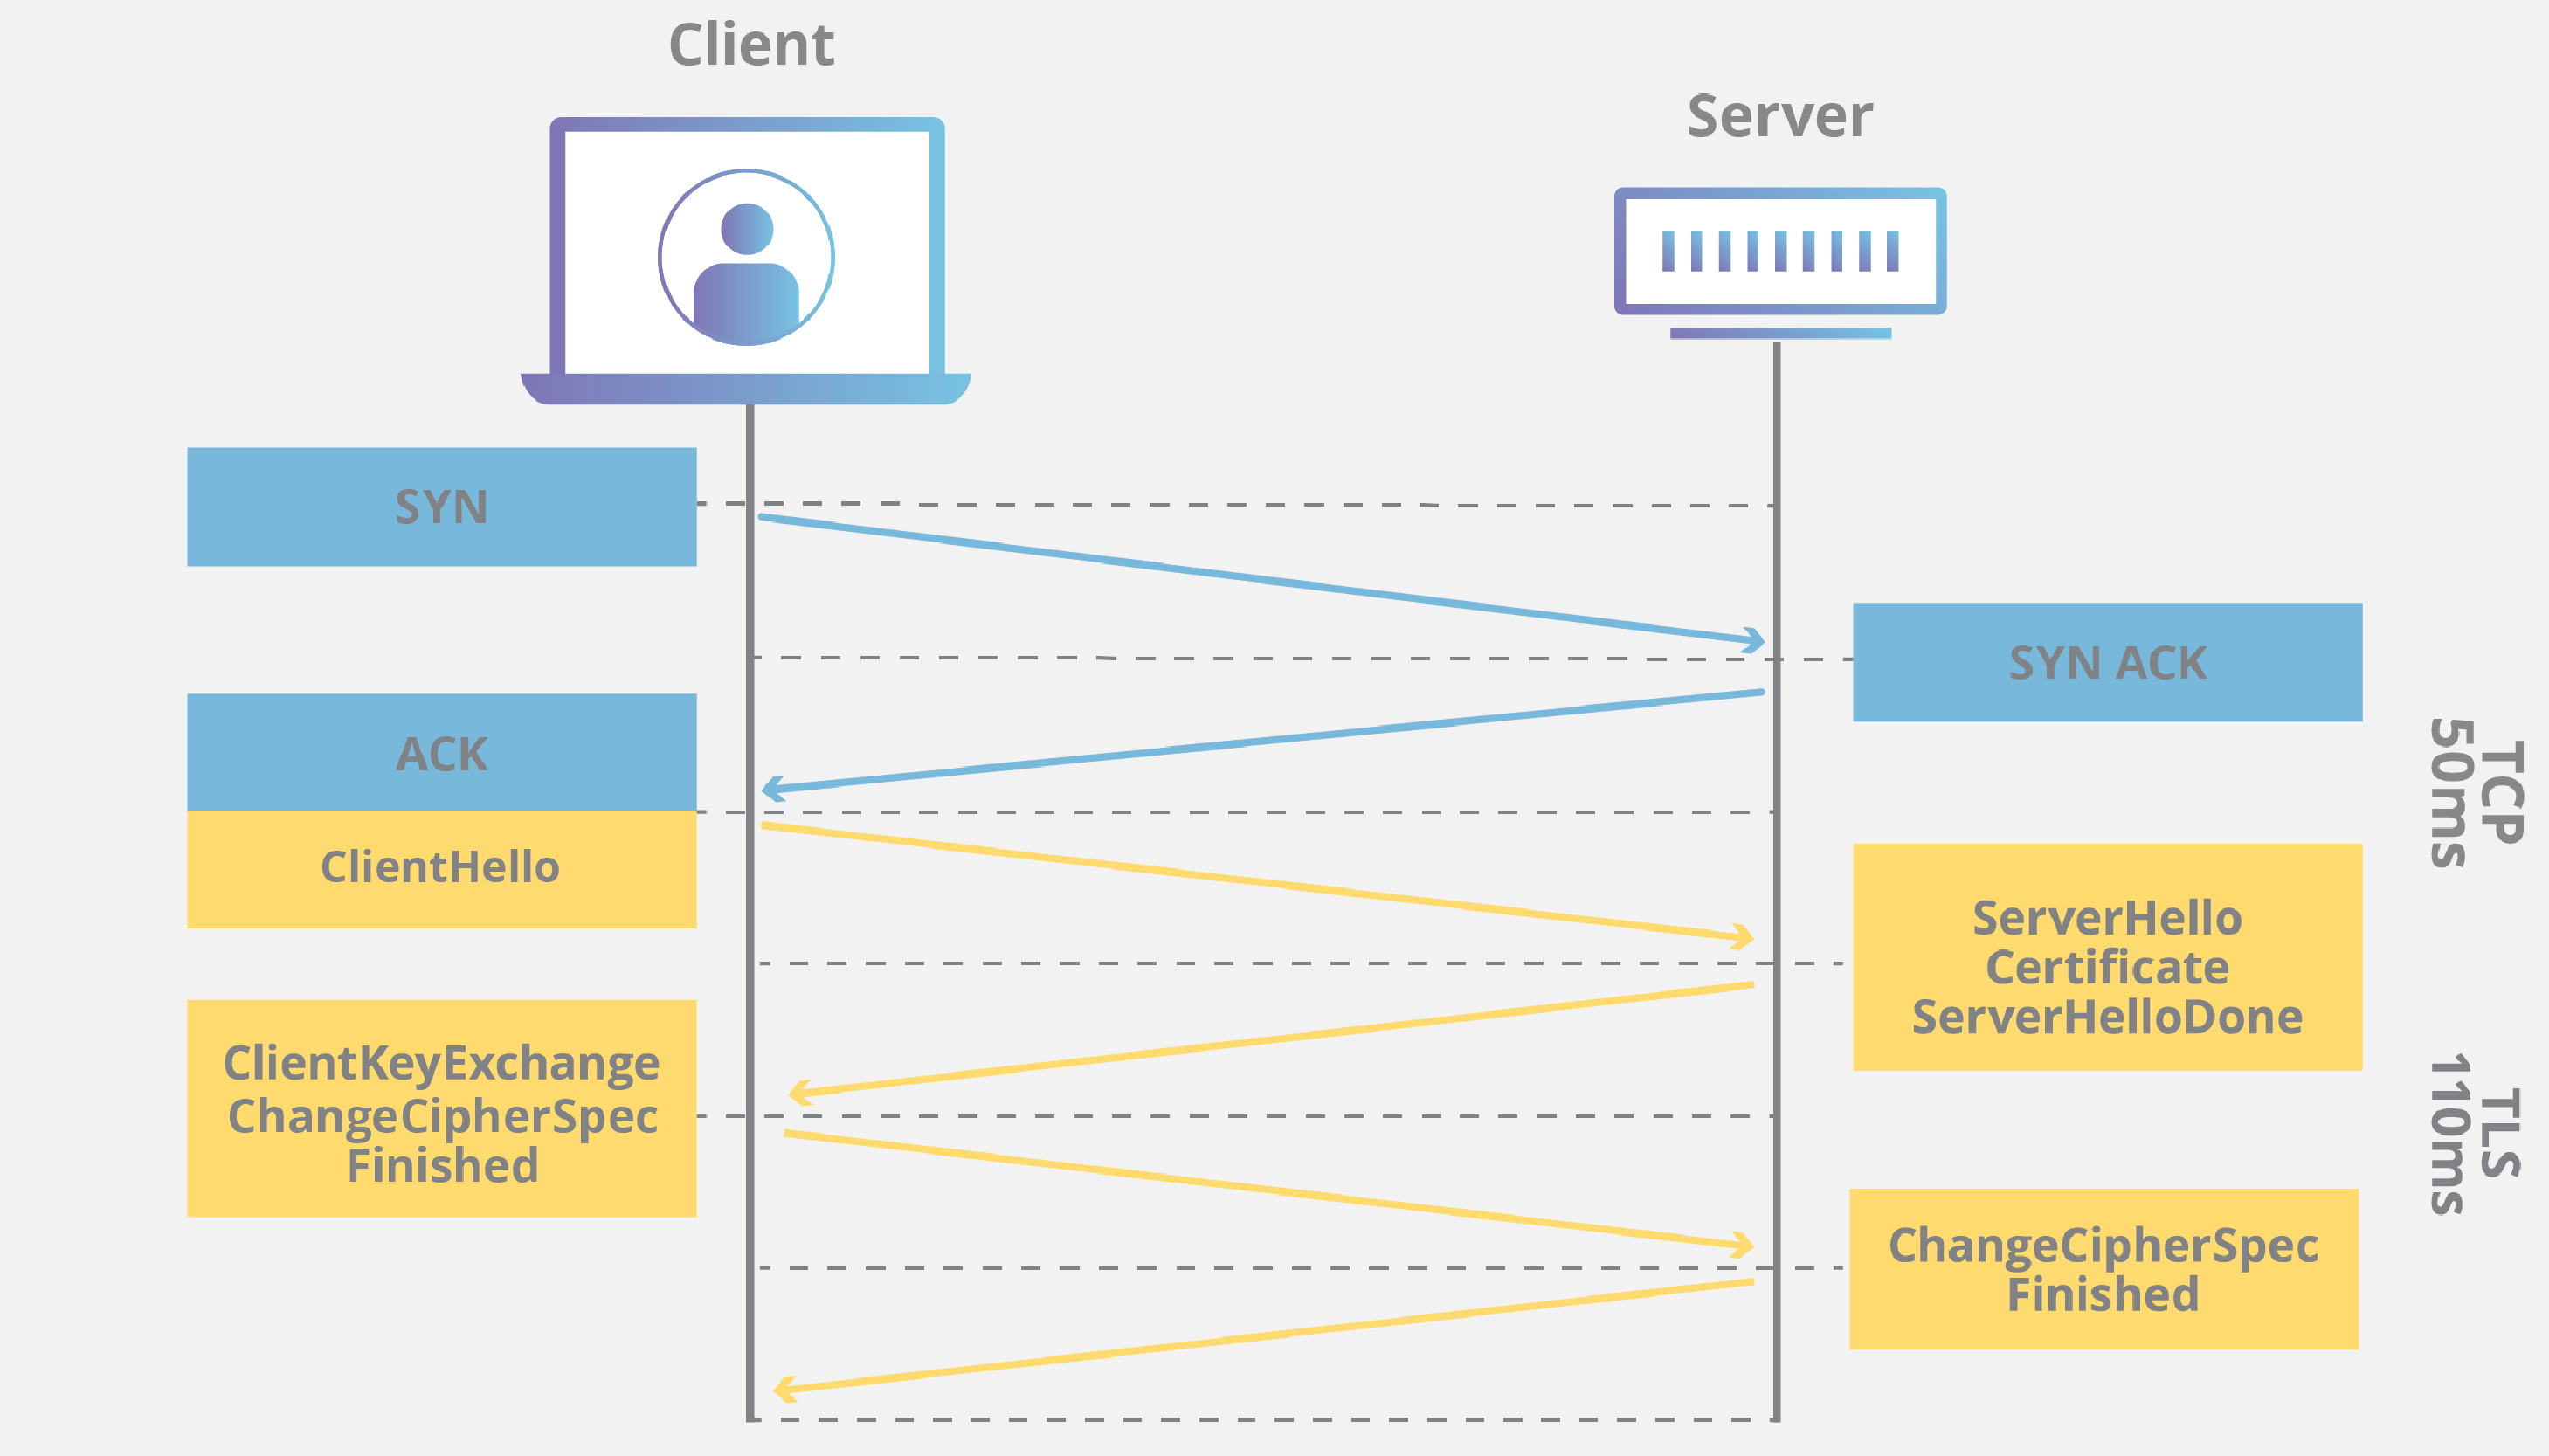
\includegraphics[width=0.7\textwidth]{img/HandshakeTLS.png}
 		\caption{Handshake TLS \cite{76}.}
 	\end{figure}
 	
 	\afterpage{\blankpage}
 	
 	\begin{thebibliography}{9}
 		\bibitem{1}
 		Wikipedia. \emph{Telefono}: https://it.wikipedia.org/wiki/Telefono
 		
 		\bibitem{2}
 		\emph{L’invenzione del telefono: più di 150 anni di storia}: https://www.tecnotrade.it/news/meucci-e-telefono-150-anni-di-storia/
 		
 		\bibitem{3}
 		Fotini-Niovi Pavlidou, Stylianos Karapantazis (2009). \emph{VoIP: A comprehensive survey on a promising technology}: https://personal.utdallas.edu/~kxs028100/Papers/VoIP.Survey.pdf
 		
 		\bibitem{4}
 		\emph{The History of VoIP and Internet Telephony}: https://getvoip.com/blog/history-of-voip/
 		
 		\bibitem{5}
 		\emph{RTMP: Real Time Messaging Protocol}: https://www.ionos.it/digitalguide/siti-web/programmazione-del-sito-web/rtmp/
 		
 		\bibitem{6}
 		\emph{Introducing OBS and RTMP support for Sendbird Live}: https://sendbird.com/blog/live-video-streaming-obs-rtmp-support
 		
 		\bibitem{7}
 		Wikipedia. \emph{WebRTC}: https://en.wikipedia.org/wiki/WebRTC
 		
 		\bibitem{8}
 		Olivier Anguenot. \emph{The WebRTC Story}: https://www.webrtc-developers.com/the-webrtc-story-part-ii/
 		
 		\bibitem{9}
 		Wikipedia. \emph{WebSocket}: https://en.wikipedia.org/wiki/WebSocket
 	
 		\bibitem{10}
 		\emph{WebRTC vs. WebSocket: Key differences and which to use}: https://ably.com/topic/webrtc-vs-websocket
 		
 		\bibitem{11}
 		\emph{WebRTC Architecture}: https://webrtc.github.io/webrtc-org/architecture/
 		
 		\bibitem{12}
 		TutorialsPoint. \emph{Webrtc Tutorial}: https://www.tutorialspoint.com/webrtc/webrtc\_tutorial.pdf
 		
 		\bibitem{13}
 		Donika Mehmeti, Linus Palmblad . \emph{Application Programming Interfaces, an exploration of their properties and what to consider during implementation}: https://www.diva-portal.org/smash/get/diva2:1685846/FULLTEXT01.pdf
 		
 		\bibitem{14}
 		Wikipedia. \emph{API}: https://en.wikipedia.org/wiki/API
 		
 		\bibitem{15}
 		\emph{What is an API (Application Programming Interface)?} : https://www.geeksforgeeks.org/what-is-an-api/
 		
 		\bibitem{16}
 		\emph{RTCPeerConnection}: https://developer.mozilla.org/en-US/docs/Web/API/RTCPeerConnection
 		
 		\bibitem{17}
 		\emph{RTCDataChannel}: https://developer.mozilla.org/en-US/docs/Web/API/RTCDataChannel
 		
 		\bibitem{18}
 		\emph{MediaStream}: https://developer.mozilla.org/en-US/docs/Web/API/MediaStream
 		
 		\bibitem{19}
 		\emph{WebRTC API}: https://developer.mozilla.org/en-US/docs/Web/API/WebRTC\_API
 		
 		\bibitem{20}
 		\emph{Differences between TCP and UDP}: https://www.geeksforgeeks.org/differences-between-tcp-and-udp/
 		
 		\bibitem{21}
 		\emph{Why you should prefer UDP over TCP for your WebRTC sessions}: https://bloggeek.me/why-you-should-prefer-udp-over-tcp-for-your-webrtc-sessions/
 		
 		\bibitem{22}
 		Wikipedia. \emph{STUN}: https://en.wikipedia.org/wiki/STUN
 		
 		\bibitem{23}
 		\emph{WebRTC TURN server: Everything you need to know}: https://www.100ms.live/blog/webrtc-turn-server
 		
 		\bibitem{24}
 		Redouane Meddane (2020). \emph{STUN TURN and ICE for NAT Traversal}
 		
 		\bibitem{25}
 		\emph{Introduction to WebRTC protocols}: https://developer.mozilla.org/en-US/docs/Web/API/WebRTC\_API/Protocols
 		
 		\bibitem{26}
 		\emph{What, Why and How (WebRTC)}: https://webrtcforthecurious.com/docs/01-what-why-and-how/
 		
 		\bibitem{27}
 		Cui Jian, Zhuying Lin (2015). \emph{Research and Implementation of WebRTC Signaling via WebSocket-based for Real-time Multimedia Communications}
 		
 		\bibitem{28}
 		\emph{RTCDataChannel - WebRTC Explained}: https://www.onsip.com/voip-resources/voip-fundamentals/rtcdatachannels
 		
 		\bibitem{29}
 		\emph{Microsoft Teams meetings on unsupported browsers}: https://learn.microsoft.com/en-us/microsoftteams/unsupported-browsers
 		
 		\bibitem{30}
 		\emph{RTCPeerConnection Support}: https://caniuse.com/?search=RTCPeerConnection
 		
 		\bibitem{31}
 		Alberto Baravaglio, Alberto Cuda, Enrico Marocco (2013). \emph{WebRTC: La nuova sfida nelle comunicazioni real-time audio/video}
 		
 		\bibitem{32}
 		\emph{WebRTC browser support on desktop and mobile}: https://bloggeek.me/webrtc-browser-support/
 		
 		\bibitem{33}
 		\emph{WebRTC Securing}: https://webrtcforthecurious.com/docs/04-securing/
 		
 		\bibitem{34}
 		Gordon H. (2022). \emph{WebRTC IP Leaks: Should You Still Be Worried?}: https://getstream.io/blog/webrtc-ip-leaks/
 		
 		\bibitem{35}
 		\emph{Verifica fughe di WebRTC}: https://surfshark.com/it/webrtc-leak-test
 		
 		\bibitem{36}
 		\emph{Benefits of using WebRTC for Online Education and eLearning}: https://www.digitalsamba.com/blog/benefits-of-using-webrtc-for-online-education-and-elearning
 		
 		\bibitem{37}
 		Wikipedia. \emph{IoT}: https://en.wikipedia.org/wiki/Internet\_of\_things
 		
 		\bibitem{38}
 		\emph{Applications of WebRTC in IoT}: https://www.iotforall.com/use-cases-for-webrtc-in-iot-applications
 		
 		\bibitem{39}
 		\emph{Powering IoT with secure real time communication}: https://rtcweb.in/powering-iot-with-secure-real-time-communication/
 		
 		\bibitem{40}
 		Antonio Preucil (2021). \emph{Using WebRTC for a browser multiplayer game}: https://dev.to/bornfightcompany/using-webtrc-for-a-browser-multiplayer-game-in-theory-59dk
 		
 		\bibitem{41}
 		Wikipedia. \emph{Cloud gaming}: https://it.wikipedia.org/wiki/Cloud\_gaming
 		
 		\bibitem{42}
 		Alberto Gonzalez (2021). \emph{WebRTC Cloud Gaming: Unboxing Stadia.}: https://webrtc.ventures/2021/02/webrtc-cloud-gaming-unboxing-stadia/
 		
 		\bibitem{43}
 		Traci Ruether (2022). \emph{RTMP vs WebRTC}: https://www.wowza.com/blog/rtmp-streaming-real-time-messaging-protocol
 		
 		\bibitem{44}
 		Wikipedia. \emph{HTTPS}: https://en.wikipedia.org/wiki/HTTPS
 		
 		\bibitem{45}
 		\emph{HLS Support}: https://caniuse.com/?search=hls
 		
 		\bibitem{46}
 		\emph{Microsoft Teams vs. Zoom} (2022): https://www.crazyegg.com/blog/microsoft-teams-vs-zoom/
 		
 		\bibitem{47}
 		\emph{Zoom piani e licenze}: https://zoom.us/it/pricing
 		
 		\bibitem{48}
 		\emph{Teams: meetings, webinars, and live events}: https://learn.microsoft.com/en-us/microsoftteams/quick-start-meetings-live-events
 		
 		\bibitem{49}
 		\emph{Microsoft forum}: https://answers.microsoft.com/en-us/msteams/forum/all/teams-is-not-supported-on-any-ios-browser/14ce2d1f-bfbe-4fde-8fde-cd0a4df1e2cb
 		
 		\bibitem{50}
 		Wikipedia. \emph{VP8}: https://en.wikipedia.org/wiki/VP8
 		
 		\bibitem{51}
 		 P. Srisuresh, Jasmine Networks, K. Egevang (2001). \emph{Traditional IP Network Address Translator (Traditional NAT)}: https://www.rfc-editor.org/rfc/rfc3022.html
 		
 		\bibitem{52}
 		Wikipedia. \emph{NAT}: https://en.wikipedia.org/wiki/Network\_Address\_Translation
 		
 		\bibitem{53}
 		Wikipedia. \emph{TLS}: https://en.wikipedia.org/wiki/Transport\_Layer\_Security
 		
 		\bibitem{54}
 		\emph{TLS Basics}: https://www.internetsociety.org/deploy360/tls/basics/	
  		
  		\bibitem{55}
  		Jay Hilotin: \emph{A brief history of the telephone}: https://gulfnews.com/world/a-brief-history-of-the-telephone-1.1603713110135
  		
  		\bibitem{56}
  		\emph{Telefono e centralino VoIP per il business, tutto quello che bisogna sapere}: 
  		https://www.iotatau.com/telefono-centralino-voip-business-hotel/
  		
  		\bibitem{57}
  		Emiliano Tomasoni: \emph{Che cos’è WebRTC ed è sicuro?}: 
  		https://blog.wildix.com/it/cose-webrtc-ed-sicuro/
  		
  		\bibitem{58}
  		Maulik Shah: \emph{WebRTC Architecture – A Layman’s Guide}: 
  		https://tragofone.com/webrtc-architecture-types-guide/
  		
  		\bibitem{59}
  		Martin Meszaros: \emph{WebRTC triangle architecture}: 
  		https://www.researchgate.net/figure/WebRTC-triangle-architecture-27\_fig3\_328334940
  		
  		\bibitem{60}
  		Martin Meszaros: \emph{WebRTC trapezoid architecture}: 
  		https://www.researchgate.net/figure/WebRTC-trapezoid-architecture-according-to-Maruschke-et-al-27-and-Alvestrand-49\_fig4\_328334940
  		
  		\bibitem{61}
  		Akshita Kumawat: \emph{What is an API (Application Programming Interface)?}:
  		https://www.geeksforgeeks.org/what-is-an-api/
  		
  		\bibitem{62}
  		Omer Sayem: \emph{STUN,TURN and ICE servers - NAT traversal for WebRTC}:
  		https://dev.to/sayem\_omer/stun-turn-and-ice-servers-nat-traversal-for-webrtc-5e29
  		
  		\bibitem{63}
  		Kavirajan ST: \emph{What is WebRTC and How to Setup STUN/TURN Server for WebRTC Communication?}:
  		https://medium.com/av-transcode/what-is-webrtc-and-how-to-setup-stun-turn-server-for-webrtc-communication-63314728b9d0
  		
  		\bibitem{64}
  		Karthikeyan S: \emph{WebRTC TURN Server: Internals and Beyond}:
  		https://web-dev.100ms.live/blog/webrtc-turn-server
  		
  		\bibitem{65}
  		\emph{Webrtc-sandbox-flutter}:
		https://github.com/lambiengcode/webrtc-sandbox-flutter?ref=flutterawesome.com
 		
 		\bibitem{66}
 		W3C: \emph{WebRTC 1.0: Real-time Communication Between Browsers}:
 		https://dev.w3.org/2011/webrtc/editor/archives/20121019/webrtc.html	
 		
 		\bibitem{67}
 		\emph{A Study of WebRTC Security}:
 		https://webrtc-security.github.io/
 		
 		\bibitem{68}
 		\emph{Cosa è un router VPN è perché ne hai bisogno? }: 		https://community.fs.com/it/blog/what-is-vpn-router-why-you-need-it.html
 		
 		\bibitem{69}
 		Dalibor Kofjač: \emph{WebRTC – the technology connecting the modern world}:
 		https://ekobit.com/blog/webrtc-the-technology-connecting-the-modern-world/
 		
 		\bibitem{70}
 		Corriere Quotidiano: \emph{Il 90\% degli italiani è favorevole all’introduzione dell’educazione finanziaria nelle scuole e l’80\% sul posto di lavoro}:
 		https://corrierequotidiano.it/scuola/il-90-degli-italiani-e-favorevole-allintroduzione-delleducazione-finanziaria-nelle-scuole-e-l80-sul-posto-di-lavoro/
 		
 		\bibitem{71}
 		Wikipedia: \emph{Telelavoro}:
 		https://it.wikipedia.org/wiki/Telelavoro
 		
 		\bibitem{72}
 		Alberto Gonzalez: \emph{WebRTC Cloud Gaming: Unboxing Stadia}:
 		https://webrtc.ventures/2021/02/webrtc-cloud-gaming-unboxing-stadia/
 		
 		\bibitem{73}
 		Dominic Kent: \emph{Microsoft Teams vs Zoom: Which Is Best For Your Business?}:
 		https://dispatch.m.io/microsoft-teams-vs-zoom/
 		 		
 		\bibitem{74}
 		\emph{VP8}:		
 		https://bloggeek.me/webrtcglossary/vp8/
 		
 		\bibitem{75}
 		\emph{Cosa è NAT e quali sono i vantaggi dei firewall NAT?}: 
 		https://community.fs.com/it/blog/what-is-nat-and-what-are-the-benefits-of-nat-firewalls.html
 		
 		\bibitem{76}
 		\emph{Cosa succede in un handshake TLS? | Handshake SSL}: https://www.cloudflare.com/it-it/learning/ssl/what-happens-in-a-tls-handshake/
 		
 		\bibitem{77}
 		\emph{MediaDevices: getUserMedia() method}: 
 		https://developer.mozilla.org/en-US/docs/Web/API/MediaDevices/getUserMedia
 		
 		\bibitem{78}
 		\emph{Creating a Self-Signed Certificate With OpenSSL}: 
 		https://www.baeldung.com/openssl-self-signed-cert
 		
 		\bibitem{79}
 		Wikipedia: \emph{Certificate Signing Request}: 
 		https://it.wikipedia.org/wiki/Certificate\_Signing\_Request
	\end{thebibliography}
 
 		\afterpage{\blankpage}
 
 	\chapter*{Ringraziamenti}
 	Infine, volevo dedicare questa ultima pagina per ringraziare tutte le persone che mi hanno sostenuto in questi anni di università, a partire dal mio relatore di tesi Andrea Piroddi che, oltre ad avermi proposto l'argomento WebRTC, è sempre stato disponibile sia ad aiutarmi nella scrittura della tesi, sia a visionare il progresso del lavoro con riunioni settimanali.$\\$ Ringrazio la mia famiglia per avermi sostenuto moralmente ed economicamente e mi abbia spronato a raggiungere questo risultato. $\\$
 	In conclusione, Ringrazio i miei amici per aver reso questa esperienza universitaria più piacevole.
\end{document}